\documentclass[10pt,twoside,leqno]{article}
% {{{-1 Preamble
\usepackage[utf8]{inputenc}
\usepackage[T1]{fontenc}
\usepackage[full]{textcomp}

\usepackage{csquotes}
\usepackage[english]{babel}

% \usepackage[urw-garamond,expert,
% uppercase=upright,greeklowercase=upright]{mathdesign}
% \usepackage[osf,swashQ]{garamondx}
% \def\kappa{\varkappa}
\usepackage{mathtools}
\mathtoolsset{mathic} % Italic correction before mathmode, works with ~'s.
% \def\mathds{\mathbb}

\usepackage{cfr-lm}
\usepackage{dsfont}  % disable this when loading mathdesign

\usepackage{microtype}
% \linespread{1.25}  % = 1.500 * fontheight
\linespread{1.388} % = 1.666 * fontheight
\usepackage[
% paper=b5paper,
nohead,nomarginpar,
% bindingoffset=.3cm,
paper=a4paper,
]{geometry}

% \raggedbottom

\usepackage{lastpage}
\usepackage{fancyhdr}
\pagestyle{fancy}
\fancyhf{}
\renewcommand{\headrulewidth}{0pt}
\fancyfoot[LE,RO]{\thepage/\pageref{LastPage}}

\usepackage{longtable}
\usepackage{booktabs}
\usepackage{tabu}

\usepackage[inline]{enumitem}
\setlist{noitemsep,nosep,listparindent=\parindent}
\setlist[itemize]{label=\guillemotright}
\setlist[enumerate,1]{ref=\thesubsection.\arabic*}
\setlist[enumerate,2]{label=\alph*.,ref=\theenumi.\alph*}
% \setlist[enumerate*]{label=(\textit{\roman*}\thinspace)}

\usepackage{cjhebrew}

\usepackage[backend=biber,doi=false,url=false,isbn=false,%
safeinputenc,style=quasialphabetic,citestyle=alphabetic]{biblatex}
\bibliography{\jobname.bib}
\defbibheading{bibliography}[\bibname]{\sectionstar{#1}}

%%% SECTION HEADINGS
\usepackage{ifthen}
\makeatletter
\renewcommand{\part}[1]{%
 \cleardoublepage%
 \vbox{\null\vskip90pt%
 \normalfont\fontsize{20pt}{30pt}\selectfont%
 \baselineskip=30pt%
 \scshape\noindent\textls*{#1}\par}%
 \addcontentsline{toc}{part}{#1}%
 \@afterindentfalse%
 \@afterheading%
}
\renewcommand{\section}[1]{%
 \vskip2\baselineskip\penalty-250%
 \refstepcounter{section}%
 \vbox{\normalfont\fontsize{12pt}{15pt}\selectfont%
  \centering\scshape\noindent\textls*{\thesection\quad#1}%
  \par}
 \nobreak
 \addcontentsline{toc}{section}{\protect\numberline{\thesection} #1}%
 \@afterindentfalse%
 \@afterheading%
} 
\newcommand{\sectionstar}[1]{%
 \vskip2\baselineskip\penalty-250
 \vbox{\normalfont\fontsize{12pt}{15pt}\selectfont%
  \centering\scshape\noindent\textls*{#1}%
  \par}
 \nobreak\vskip15pt
 \@afterindentfalse%
 \@afterheading%
} 
\renewcommand{\paragraph}[1]{\par\bigskip\refstepcounter{subsection}%
 {\normalfont\normalsize\scshape\noindent\thesubsection%
 \ifthenelse{\equal{#1}{}}%
 {}%
 {\ \textls{#1.}}%
 \ ---}%
}
\newcommand{\readme}{\par\vskip\baselineskip%
 {\normalfont\normalsize\scshape\noindent%
  \textls{Readme.}\ ---}
}
\renewcommand\tableofcontents{%
 \sectionstar{\contentsname}%
 \@starttoc{toc}%
}
\renewcommand*\l@part[2]{%
 \addvspace{15pt \@plus\p@}%
 \noindent{\leavevmode%
  \scshape\textls{#1\qquad#2}%
 }\par\nobreak%
}
\renewcommand*\l@section[2]{%
 \setlength\@tempdima{\parindent}%
 \noindent
 {\leavevmode%
  \hskip\parindent#1\qquad#2%
 }\par\nobreak%
}
\makeatother

%%% MATH PACKAGES
\usepackage{amsmath,amssymb}  % disable when using mathdesign
\usepackage{mathrsfs}         % disable when using mathdesign
\usepackage{mathabx}

\usepackage[thmmarks,amsmath]{ntheorem}
\usepackage{thmtools}

\numberwithin{equation}{subsection}

\declaretheoremstyle[headformat=swapnumber,headpunct={.\ ---},%
headfont=\normalfont\scshape\lsstyle,bodyfont=\itshape,%
spaceabove=0pt,spacebelow=0pt,%
preheadhook={\bigskip}]{theorem}
\declaretheorem[style=theorem,sibling=subsection]{theorem}
\declaretheorem[style=theorem,sibling=subsection]{proposition}
\declaretheorem[style=theorem,sibling=subsection]{lemma}
\declaretheorem[style=theorem,sibling=subsection]{corollary}
\declaretheorem[style=theorem,sibling=subsection]{conjecture}

\declaretheoremstyle[headformat=swapnumber,headpunct={.\ ---},%
headfont=\normalfont\scshape\lsstyle,bodyfont=\normalfont,%
spaceabove=0pt,spacebelow=0pt,%
preheadhook={\bigskip}]{definition}
\declaretheorem[style=definition,sibling=subsection]{definition}
\declaretheorem[style=definition,sibling=subsection]{exercise}
\declaretheorem[style=definition,sibling=subsection]{example}
\declaretheorem[style=definition,sibling=subsection]{remark}
\declaretheorem[style=definition,sibling=subsection]{notation}
\declaretheorem[style=definition,sibling=subsection]{construction}

\declaretheoremstyle[headpunct={\!.},headfont=\itshape,bodyfont=\normalfont,%
qed=\ensuremath{\square},spaceabove=0pt,spacebelow=0pt]{proof}
\declaretheoremstyle[headpunct={\!.},headfont=\itshape,bodyfont=\normalfont,%
qed=\ensuremath{\square},spaceabove=0pt,spacebelow=0pt]{nonumberproof}
\declaretheorem[style=proof,numbered=no]{proof}

\declaretheoremstyle[headformat=swapnumber,headpunct={.\ ---},%
headfont=\itshape,bodyfont=\normalfont,qed=\ensuremath{\square},%
spaceabove=0pt,spacebelow=0pt,%
preheadhook={\bigskip}]{nproof}
\declaretheorem[style=nproof,sibling=subsection,name=Proof]{nproof}

% \let\qed\relax
% \usepackage{pf2}
% \pfkeywords{jmc}

\usepackage{cleveref}
\crefname{condition}{condition}{conditions}
\crefname{conjecture}{conjecture}{conjectures}
\crefname{construction}{construction}{constructions}
\crefname{corollary}{corollary}{corollaries}
\crefname{diagram}{diagram}{diagrams}
\crefformat{subsection}{\S#2#1#3}
\crefformat{enumi}{\S#2#1#3}
\crefformat{nproof}{\S#2#1#3}
\creflabelformat{equation}{#2#1#3}

%%% MATH MACROS
\newcommand{\id}{\textnormal{id}}

\newcommand{\into}{\hookrightarrow}
\newcommand{\onto}{\twoheadrightarrow}
\newcommand{\longto}{\longrightarrow}
\newcommand{\longinto}{\lhook\joinrel\longrightarrow}

\renewcommand{\Im}{\textnormal{Im}}

\newcommand{\colim}{\mathop{\textnormal{colim}}}

\newcommand{\Hom}{\textnormal{Hom}}
\newcommand{\End}{\textnormal{End}}
\newcommand{\Isom}{\textnormal{Isom}}
\newcommand{\Inn}{\textnormal{Inn}}
\newcommand{\Aut}{\textnormal{Aut}}
\newcommand{\Out}{\textnormal{Out}}
\newcommand{\iHom}{\underline{\Hom}}
\newcommand{\iEnd}{\underline{\End}}
\newcommand{\iIsom}{\underline{\Isom}}
\newcommand{\iInn}{\underline{\Inn}}
\newcommand{\iAut}{\underline{\Aut}}
\newcommand{\iOut}{\underline{\Out}}

\newcommand{\Mat}{\textnormal{Mat}}
\newcommand{\Sym}{\textnormal{Sym}}

\newcommand{\Fil}{\textnormal{Fil}}

\newcommand{\dual}[1]{\check{#1}}

\newcommand{\NN}{\mathbb{N}}
\newcommand{\ZZ}{\mathbb{Z}}
\newcommand{\QQ}{\mathbb{Q}}
\newcommand{\QQbar}{\bar{\QQ}}
\newcommand{\QQl}{\QQ_{\ell}}
\newcommand{\QQlbar}{\QQbar_{\ell}}
\newcommand{\QQp}{\QQ_{p}}
\newcommand{\QQpbar}{\QQbar_{p}}
\newcommand{\BB}{\mathrm{B}}
\newcommand{\RR}{\mathbb{R}}
\newcommand{\CC}{\mathbb{C}}
\newcommand{\HQ}{\mathbb{H}}
\newcommand{\FF}{\mathbb{F}}
\newcommand{\FFp}{\FF_{p}}
\newcommand{\FFq}{\FF_{q}}
\newcommand{\FFqbar}{\bar{\FF}_{q}}
\newcommand{\Adele}{\mathbb{A}}
\newcommand{\fin}{\textnormal{f}}

\newcommand{\primes}{\mathscr{L}}

\newcommand{\Spec}{\textnormal{Spec}}

\newcommand{\DelS}{\mathbb{S}}
\newcommand{\Sh}{\textnormal{Sh}}
\newcommand{\mSh}{\mathscr{S}}
\newcommand{\DD}{\mathbb{D}}
\newcommand{\mcG}{\mathcal{G}}
\newcommand{\Kmpt}{\mathcal{K}}
\newcommand{\Sds}{\mathfrak{H}^{\pm}}
\newcommand{\AV}{\mathscr{A}}
\newcommand{\Ag}{\AV_{g}}

\newcommand{\Gal}{\textnormal{Gal}}

% \newcommand{\HH}{\textnormal{H}}
% \newcommand{\Hhom}{\HH_{\textnormal{hom}}}
\newcommand{\HdR}{\HH_{\dR}}
% \newcommand{\Hl}{\HH_{\ell}}
% \newcommand{\Hp}{\HH_{p}}
% \newcommand{\Hlambda}{\HH_{\lambda}}
% \newcommand{\HB}{\HH_{\textnormal{B}}}
% \newcommand{\Hsigma}{\HH_{\sigma}}

% \newcommand{\GG}{\textnormal{G}}
% \newcommand{\Gl}{\GG_{\ell}}
% \newcommand{\Glc}{\Gl^{\circ}}
% \newcommand{\GB}{\GG_{\textnormal{B}}}
% \newcommand{\Gsigma}{\GG_{\sigma}}
% \newcommand{\Gmot}[1]{\GG_{\textnormal{mot},#1}}
% \newcommand{\Gmots}{\Gmot{\sigma}}
% \newcommand{\Gmotl}{\Gmot{\ell}}
% \newcommand{\GmotB}{\Gmot{\textnormal{B}}}

% \newcommand{\Zl}{\textnormal{Z}_{\ell}}
% \newcommand{\Zlc}{\Zl^{\circ}}
% \newcommand{\ZB}{\textnormal{Z}_{\textnormal{B}}}
% \newcommand{\Zsigma}{\textnormal{Z}_{\sigma}}
% \newcommand{\Zmot}[1]{\textnormal{Z}_{\textnormal{mot},#1}}
% \newcommand{\Zmots}{\Zmot{\sigma}}
% \newcommand{\Zmotl}{\Zmot{\ell}}

\newcommand{\BdR}[1]{\textnormal{B}_{\dR,#1}}
\newcommand{\HT}{\textnormal{HT}}
\newcommand{\BHT}[1]{\textnormal{B}_{\textnormal{HT},#1}}
\newcommand{\gr}{\textnormal{gr}}

\newcommand{\Vect}{\textnormal{Vect}}
\newcommand{\grVect}{\textnormal{grVect}}
\newcommand{\Filt}{\textnormal{Filt}}
\newcommand{\Rep}{\textnormal{Rep}}
\newcommand{\QHS}{\QQ\textnormal{HS}}

\makeatletter
\def\cpwith[#1]#2{\textnormal{c.p.}_{#1}(#2)}
\def\cpwithout#1{\textnormal{c.p.}(#1)}
\def\cp{\@ifnextchar[{\cpwith}{\cpwithout}}
\makeatother
\makeatletter
\def\Gmwith[#1]{\mathbb{G}_{\textnormal{m},#1}}
\def\Gmwithout{\mathbb{G}_{\textnormal{m}}}
\def\Gm{\@ifnextchar[{\Gmwith}{\Gmwithout}}
\makeatother
\newcommand{\GL}{\textnormal{GL}}
\newcommand{\SL}{\textnormal{SL}}
\newcommand{\PGL}{\textnormal{PGL}}
\newcommand{\UU}{\textnormal{U}}
\newcommand{\SU}{\textnormal{SU}}
\newcommand{\GU}{\textnormal{GU}}
\newcommand{\PGU}{\textnormal{PGU}}
\newcommand{\OO}{\textnormal{O}}
\newcommand{\SO}{\textnormal{SO}}
\newcommand{\GO}{\textnormal{GO}}
\newcommand{\PGO}{\textnormal{PGO}}
\newcommand{\Spin}{\textnormal{Spin}}
\newcommand{\CSpin}{\textnormal{CSpin}}
\newcommand{\PSpin}{\textnormal{PSpin}}
\newcommand{\Sp}{\textnormal{Sp}}
\newcommand{\CSp}{\textnormal{CSp}}
\newcommand{\PCSp}{\textnormal{PCSp}}
\newcommand{\Lie}{\textnormal{Lie}}

\newcommand{\Char}{\textnormal{X}^{*}}
\newcommand{\Cochar}{\textnormal{X}_{*}}

\newcommand{\Dyn}{\textnormal{Dyn}}

% \newcommand{\mfsl}{\mathfrak{sl}}
% \newcommand{\mfso}{\mathfrak{so}}

\newcommand{\Cliff}{\textnormal{Cl}}
% \newcommand{\spin}{\textnormal{spin}}

% \newcommand{\St}{\textnormal{St}}

\newcommand{\ab}{\textnormal{ab}}
\newcommand{\der}{\textnormal{der}}
\newcommand{\ad}{\textnormal{ad}}
\newcommand{\ha}{\textnormal{ha}}

\newcommand{\SmPr}{\textnormal{SmPr}}
\newcommand{\Fib}{\textnormal{Fib}}
\newcommand{\Mod}{\textnormal{Mod}}
\newcommand{\Proj}{\textnormal{Proj}}

\newcommand{\an}{\textnormal{an}}
\newcommand{\cl}{\textnormal{cl}}

\newcommand{\dR}{\textnormal{dR}}
\newcommand{\et}{\textnormal{\'{e}t}}
\newcommand{\sing}{\textnormal{sing}}

\newcommand{\HH}{\textnormal{H}}
\newcommand{\Hl}{\HH_{\ell}}
\newcommand{\Hp}{\HH_{p}}
\newcommand{\Hlambda}{\HH_{\lambda}}
\newcommand{\HB}{\HH_{\textnormal{B}}}
\newcommand{\HLambda}{\HH_{\Lambda}}

\newcommand{\Zar}{\textnormal{Zar}}

\newcommand{\Mot}{\textnormal{Mot}}

\newcommand{\Zentrum}{\textnormal{Z}}
\newcommand{\GG}{\textnormal{G}}
\newcommand{\GB}{\GG_{\textnormal{B}}}
\newcommand{\Gp}{\GG_{p}}
\newcommand{\Gpc}{\Gp^{\circ}}
\newcommand{\Gl}{\GG_{\ell}}
\newcommand{\Glc}{\Gl^{\circ}}
\newcommand{\Glambda}{\GG_{\lambda}}
\newcommand{\Glambdac}{\Glambda^{\circ}}

\newcommand{\HS}{\textnormal{HS}}

\newcommand{\alg}{\textnormal{alg}}
\newcommand{\tra}{\textnormal{tra}}

\newcommand{\Res}{\textnormal{Res}}
\newcommand{\Nm}{\textnormal{Nm}}
\newcommand{\trace}{\textnormal{tr}}
\newcommand{\rk}{\textnormal{rk}}
\renewcommand{\det}{\textnormal{det}}
\newcommand{\res}{\textnormal{res}}

\newcommand{\chrc}{\textnormal{char}}

\newcommand{\Tangen}[1]{\langle #1 \rangle^{\otimes}}
\newcommand{\Val}{\textnormal{Val}}

\newcommand{\tr}{\textsc{tr}}
\newcommand{\cm}{\textsc{cm}}

\newcommand{\MTC}{\textnormal{MTC}}

\newcommand{\rotatesim}{\rotatebox{90}{$\sim$}}

\newcommand{\Sigmacmpt}{\Sigma_{\textnormal{c}}}
\newcommand{\Sigmanc}{\Sigma_{\textnormal{nc}}}

\usepackage{tikz}
\usetikzlibrary{calc}
\usetikzlibrary{cd,positioning,shapes}
\usetikzlibrary{decorations.pathmorphing}
\usetikzlibrary{decorations.markings}


%%%%%%%%%%%%%% Macros for Dynkin diagrams %%%%%%%%%%%%%%
\newcommand{\dynkinradius}{.04cm}
\newcommand{\dynkinstep}{.35cm}
\newcommand{\dynkinnode}[2]{\fill (\dynkinstep*#1,\dynkinstep*#2) circle (\dynkinradius);}
\newcommand{\dynkinXsize}{1.5}
\newcommand{\dynkinnodespecial}[2]{
 \draw[thick] (#1*\dynkinstep-\dynkinXsize,#2*\dynkinstep-\dynkinXsize) -- (#1*\dynkinstep+\dynkinXsize,#2*\dynkinstep+\dynkinXsize);
 \draw[thick] (#1*\dynkinstep-\dynkinXsize,#2*\dynkinstep+\dynkinXsize) -- (#1*\dynkinstep+\dynkinXsize,#2*\dynkinstep-\dynkinXsize);
}
\newcommand{\dynkinedge}[4]{\draw[thin] (\dynkinstep*#1,\dynkinstep*#2) -- (\dynkinstep*#3,\dynkinstep*#4);}
\newcommand{\dynkinnodes}[4]{\draw[dotted] (\dynkinstep*#1,\dynkinstep*#2) -- (\dynkinstep*#3,\dynkinstep*#4);}
\newcommand{\dynkindoubleedge}[4]{\draw[double,postaction={decorate}] (\dynkinstep*#1,\dynkinstep*#2) -- (\dynkinstep*#3,\dynkinstep*#4);}

\newenvironment{dynkin}{\begin{tikzpicture}[decoration={markings,mark=at position 0.7 with {\arrow{>}}}]}
 {\end{tikzpicture}}
%%%%%%%%%%%%%% End of macros for Dynkin diagrams %%%%%%%%%%%%%%


\def\title{The Mumford--Tate conjecture for products of abelian varieties}
\def\author{Johan Commelin}

\usepackage{datetime}
\def\date{\dayofweekname{\day}{\month}{\year},
 the \ordinaldate{\day} of \monthname, \number\year}
% -}}}1
\begin{document}
% {{{-1 Title
\begin{center}\Large\scshape
\textls*{\title}
\end{center}

\medskip

\noindent\textit{by} \quad \author \hfill \date

\vskip3\baselineskip

% \tableofcontents
% -}}}1

\section{Introduction} % {{{-1

\paragraph{} % {{{-2
Let $A$~be an abelian variety over a number field $K \subset \CC$.
If $\ell$ is prime number,
we write $\Hl^1(A)$ for the $\ell$-adic cohomology group
$\HH_{\et}^1(A_{\bar k}, \QQl)$;
we write $\HB^1(A)$
for the singular cohomology group $\HH_{\sing}^1(A(\CC), \QQ)$.
There is a natural isomorphism $\Hl^1(A) \cong \HB^1(A) \otimes \QQl$.

The group $\Hl^1(A)$ carries a Galois representation
$\rho_\ell \colon \Gal(\bar k/k) \to \Aut(\Hl^1(A))$,
while the Hodge structure on $\HB^1(A)$ may be described
by a representation $\rho \colon \GB(A) \to \Aut(\HB^1(A))$,
where $\GB(A)$ is the so called \emph{Mumford--Tate group} of~$A$.
(See \cref{HS} for the definition.)

Write $\Gl(A)$ for the Zariski closure of the image of~$\rho_\ell$,
and $\Glc(A)$ for the connected component of the identity of~$\Gl(A)$.
The \emph{Mumford--Tate conjecture} expresses the expectation that
the isomorphism $\Hl^1(A) \cong \HB^1(A) \otimes \QQl$
identifies $\Glc(A)$ with~$\GB(A) \otimes \QQl$.
This conjecture is still wide open,
but see \cite{Mo17} for a recent overview of the state of the art.

\paragraph{Main theorem} % {{{-2
The goal of this article is \cref{mtcaxa}:

\medskip

{\narrower\it\noindent
 Let $A_1$ and~$A_2$ be two abelian varieties
 over a finitely generated field $K \subset \CC$.
 Assume that the Mumford--Tate conjecture is true for $A_1$ and~$A_2$.
 Then the Mumford--Tate conjecture is true for $A_1 \times A_2$.
 \par}

\begin{remark} % {{{-2
 Observe that the conclusion of the theorem
 is not a formal consequence of the assumption:
 Suppose that $G'$ is a group, with two representations
 $\rho_1 \colon G' \to \Aut(V_1)$
 and
 $\rho_2 \colon G' \to \Aut(V_2)$.
 Let $G_1$ (resp.~$G_2$) be the image of~$\rho_1$ (resp.~$\rho_2$).
 Write $\rho$ for $\rho_1 \oplus \rho_2$,
 and let $G$ be the image of~$\rho$.
 Then $G$ is a subgroup of $G_1 \times G_2$,
 and the projection of~$G$ onto $G_1$ (and~$G_2$)
 is surjective.
 However, $G \subset G_1 \times G_2$
 may be anything, ranging from the diagonal
 (\emph{e.g.}, if $V_1 \cong V_2$)
 to the full product
 (\emph{e.g.}, if $G_1$ and $G_2$ are simple and non-isomorphic).
 
 In the context of the main theorem we have
 \[
  \Glc(A_1 \times A_2) \subset \Glc(A_1) \times \Glc(A_2)
  \cong (\GB(A_1) \times \GB(A_2)) \otimes \QQl
  \supset \GB(A_1 \times A_2) \otimes \QQl,
 \]
 and there is no \emph{a priori} formal reason why
 $\Glc(A_1 \times A_2)$ should be the same subgroup as
 $\GB(A_1 \times A_2) \otimes \QQl$.
\end{remark}

\begin{remark}
 Vasiu~\cite{Va08} proves a similar result to \cref{mtcaxa}
 although he has to exclude the case where $A_1$ or~$A_2$
 has a Mumford--Tate group with a simple factor of type~$D_4^\HQ$.
 His proof is long and very technical,
 and I do not claim to fully grasp the details.
 His global strategy is similar to the one employed below;
 and the reason that we can now prove the stronger claim
 is mostly due to the results of~\cite{Co17} (building on~\cite{Kisin_modp}).
\end{remark}

\paragraph{Strategy of the proof} % {{{-2
\label{strategy}

\begin{enumerate}
 \item As a first step, we linearise the category of abelian varieties,
  into so called \emph{abelian motives} (in the sense of Andr\'e~\cite{An95},
  or equivalently motives for absolute Hodge cycles).
  We obtain a semisimple Tannakian category,
  allowing us to apply the toolkit of representation theory of reductive groups.
 \item From work of several people (notably Piatetski-Shapiro,
  Deligne, Andr\'e, and Faltings) we know that for any abelian motive~$M$
  the group $\Glc(M)$ is reductive, and $\Glc(M) \subset \GB(M) \otimes \QQl$.
 \item We then prove that the connected component of the centre of~$\Glc(A)$ is
  isomorphic to the connected component of the centre of~$\GB(A) \otimes \QQl$.
  For this we employ \emph{CM~motives},
  and reduce the claim to the Mumford--Tate conjecture for CM~abelian varieties,
  for which the statement is known by work of Pohlmann~\cite{Pohl68}.
 \item The next step consists of replacing the abelian variety $A_i$ ($i = 1,2$)
  by the motive~$M_i$ that corresponds---via the Tannakian formalism---with
  the adjoint representation of $\GB(A_i)^\ad$.
  It suffices to prove the Mumford--Tate conjecture for $M_1 \oplus M_2$.
 \item By general considerations,
  we may assume that $M_1$ and~$M_2$ are irreducible motives.
  In particular, the Mumford--Tate groups~$\GB(M_1)$ and~$\GB(M_2)$
  are $\QQ$-simple adjoint groups.
  In addition, we assume that
  $\Glc(M_1 \oplus M_2) \subsetneq \Glc(M_1) \times \Glc(M_2)$.
 \item Using results from~\cite{Co17} we show that $\Hl(M_1) \cong \Hl(M_2)$,
  for all prime numbers~$\ell$,
  and we deduce that there is a canonical isomorphism
  $\End(M_1) \cong \End(M_2)$.
 \item The remainder of the proof consists of applying
  a construction of Deligne to~$M_1$ and~$M_2$
  that is reminiscent of the Kuga--Satake construction.
  As a result we acquire to abelian varieties~$\tilde A_1$ and~$\tilde A_2$,
  and our job is to show that the isomorphism $\Hl(M_1) \cong \Hl(M_2)$
  lifts to an isomorphism $\Hl^1(\tilde A_1) \cong \Hl^1(\tilde A_2)$.
  Once that is done,
  we apply Faltings's theorem, to deduce $\tilde A_1 \sim \tilde A_2$
  which implies $\GB(\tilde A_1) \cong \GB(\tilde A_2)$.
  In particular $\GB(M_1 \oplus M_2) \subset \GB(M_1) \times \GB(M_2)$
  is the diagonal,
  and therefore $\Glc(M_1 \oplus M_2) \cong \GB(M_1 \oplus M_2) \otimes \QQl$.
  Hence we win!
\end{enumerate}


\paragraph{Acknowledgements} % {{{-2
My warmest thanks go to my supervisor Ben Moonen.
Our countless discussions and his many detailed explanations and corrections
have been of immense importance for this article.
I also thank Rutger Noot for a very inspiring discussion of this subject.
This article also benefited from the extensive feedback on my PhD~thesis
that I received from Anna Cadoret, Pierre Deligne, Bas Edixhoven,
Milan Lopuha\"a, Rutger Noot, and Lenny Taelman.
I thank Netan Dogra, Milan Lopuha\"a, Joost Nuiten, and Salvatore Floccari
for their interest and useful comments.

\section{Adjoint objects in Tannakian categories} % {{{-1

\readme % {{{-2
In representation theory the adjoint representation is very important.
Tannakian categories behave like
the category of representations of an affine group scheme.
We define \emph{adjoint} objects in Tannakian categories
and study a bit of their properties.

This ties into the the proof of the main theorem
because we will replace abelian varieties~$A$ by the motive
that corresponds to the adjoint representation of the
motivic Galois group of~$A$.
(See also the strategy in \cref{strategy}.)

\paragraph{} % {{{-2
Let $T$ be a Tannakian category over a field~$Q$ of characteristic~$0$.
For a $Q$-algebra~$R$, let $\Fib(T)_R$ be the groupoid of
fibre functors $T \to \Mod_R$,
that is, $Q$-linear tensor functors that are faithful and exact
that take values in the subcategory $\Proj_R \subset \Mod_R$
of finitely generated projective $R$-modules.
It turns out that $\Fib(T)$ is an algebraic stack over~$\QQ$.
In fact, if $\alpha \colon Q \to R$ is a $Q$-algebra,
and $\omega \colon T \to \Mod_R$ is a fibre functor,
then the stack $\alpha^*\Fib(T)$ is isomorphic to $\BB G = [\Spec(R)/G]$,
where $G$ is the affine group scheme $\iAut^\otimes(\omega)$ over~$R$.
This observation makes $\Fib(T)$ into a gerbe
(together with the fact that such fibre functors exist).

A representation of~$\Fib(T)$ is a cartesian functor $\Fib(T) \to \Proj$,
in other words, a collection of functors $\Fib(T)_R \to \Proj_R$
that is functorial in~$R$.
The category of representations of~$\Fib(T)$ is denoted $\Rep(\Fib(T))$,
and the evaluation functor $T \to \Rep(\Fib(T))$,
given by $V \mapsto (\omega \mapsto \omega(V))$ is an equivalence.
(This is one half of the statement of Tannaka duality.)

\begin{definition} % {{{-2
 Let $T$ be a Tannakian category over a field~$Q$ of characteristic~$0$.
 Assume that $T$ is finitely generated (hence generated by one object).
 The \emph{adjoint object} in~$T$ is the object
 (well-defined up to isomorphism)
 given by the collection of functors
 $\Fib(T)_R \to \Proj_R, \omega \mapsto \Lie(\iAut^\otimes(\omega))$.
 (Since $T$ is finitely generated,
 the group scheme $\iAut^\otimes(\omega)$ is of finite type,
 and therefore $\Lie(\iAut^\otimes(\omega))$ is finitely generated.)
\end{definition}

\begin{notation} % {{{-2
 Let $T$ be a Tannakian category over a field~$Q$ of characteristic~$0$.
 If $V$ is an object of~$T$,
 then $V^\ad$ denotes the adjoint object
 of the Tannakian subcategory $\Tangen{V} \subset T$ generated by~$V$.
\end{notation}

\paragraph{} % {{{-2
Let $T$ be a Tannakian category over a field~$Q$ of characteristic~$0$.
If $V$ is an object in~$T$,
define a sequence of objects by $V^{(0)} = V$,
and $V^{(i+1)} = (V^{(i)})^\ad$ for $i \in \ZZ_{\ge0}$.
Observe that for $i \ge 1$ the object~$V^{(i+1)}$ is a quotient of~$V^{(i)}$,
and therefore $\dim V^{(i+1)} \le \dim V^{(i)}$.
Since $V$ is finite-dimensional
this sequence stabilises at an object $V^{(\infty)}$.

\begin{definition} % {{{-2
 Retain the notation of the previous paragraph.
 We call the object $V^{(\infty)}$ the \emph{hyperadjoint object}
 associated with~$V$, and we denote it with~$V^\ha$.
 We say that an object $V \in T$ is \emph{hyperadjoint} if $V \cong V^\ha$
 (or equivalently, if $V \cong V^\ad$).
\end{definition}

\section{Hodge structures} \label{HS} % {{{-1

\readme % {{{-2
We start with a section on Hodge structures.
Following \cite{Del_ShimVar} we use the notion of
fractional Hodge structures,
because it will prove useful in understanding
Deligne's construction (\cref{delignes-construction}).

\begin{definition} % {{{-2
 Let $R \subset \RR$ be a subring (typically $\ZZ$,~$\QQ$, or~$\RR$).
 A \emph{fractional pre-Hodge structure} over~$R$
 consists of a free $R$-module~$V$ of finite rank,
 and a decomposition
 \[
  V \otimes \CC \cong \bigoplus_{p,q \in \QQ} V^{p,q}
 \]
 over~$\CC$, such that $V^{p,q} = \overline{V^{q,p}}$.
\end{definition}

\paragraph{} % {{{-2
Let $V$ be a fractional pre-Hodge structure over a ring $R \subset \RR$.
For $p,q \in \QQ$, we denote with $h^{p,q}(V)$ the dimension of $V_n^{p,q}$.
We say that $V$ is \emph{pure} of \emph{weight}~$n \in \QQ$
if $h^{p,q}(V) \ne 0 \implies p + q = n$.
A \emph{fractional Hodge structure} is a fractional pre-Hodge structure
that is the direct sum of pure fractional pre-Hodge structures.
A \emph{pre-Hodge structure}~$V$ (without the adjective \emph{fractional})
is a fractional pre-Hodge structure
for which $h^{p,q}(V) \ne 0 \implies p,q \in \ZZ$.
If $V$ is both a fractional Hodge structure and a pre-Hodge structure,
then $V$ is a \emph{Hodge structure}, in the classical sense of the word.

\paragraph{} % {{{-2
Let $\DelS$ denote the Deligne torus~$\Res_{\CC/\RR} \Gm$.
Recall that a Hodge structure over~$R$ is completely described
by a representation $h \colon \DelS \to \GL(V)_\RR$, as follows:
for $z \in \DelS(\CC)$ and $v \in V_n^{p,q}$
we put $h(z) \cdot v = z^{-p}\bar z^{-q}v$.
Composing $h$ with the map $\DelS \to \DelS, x \mapsto x^k$
amounts to relabeling $V_n^{p,q}$ as $V_{kn}^{kp,kq}$.

Put $\tilde \DelS = \lim_\NN \DelS$,
where $\NN$ is ordered by divisibility,
and for $m | n$, we take the transition map $\DelS \to \DelS$
given by $x \mapsto x^{n/m}$.
A fractional pre-Hodge structure is then described by a representation
$h \colon \tilde \DelS \to \GL(V)_\RR$.

\begin{definition} % {{{-2
 Let $V$ be a fractional pre-Hodge structure over a ring $R \subset \RR$.
 The \emph{Mumford--Tate group} of~$V$
 is the smallest algebraic subgroup $\GB(V) \subset \GL(V)$ over~$R$
 such that $h \colon \tilde\DelS \to \GL(V)_\RR$
 factors through $\GB(V)_\RR \subset \GL(V)_\RR$.
\end{definition}

\begin{lemma} % {{{-2
 Let $V$ be a fractional pre-Hodge structure over a ring $R \subset \RR$.
 The Mumford--Tate group of~$V$ is a torus
 if and only if
 $V$ is a free module of rank~$1$ over a commutative
 semisimple algebra $E \subset \End_{\HS}(V)$.
\end{lemma}

\begin{definition} % {{{-2
 \label{cm-hodge-structure}
 A fractional pre-Hodge structure~$V$ over a ring $R \subset \RR$
 is called \emph{of CM~type}
 (or a \emph{fractional CM~pre-Hodge structure})
 if the Mumford--Tate group $\GB(V)$ is a torus.
\end{definition}

\begin{lemma} % {{{-2
 \label{cm-hs-cat}
 The subcategory of (classical) CM~Hodge structures over~$\QQ$
 is a Tannakian subcategory
 generated by Hodge structures of the form $\HB^1(A,\QQ)$
 where $A$ is a complex abelian variety of CM~type.
\end{lemma}

\section{Abelian motives} % {{{-1

\readme % {{{-2
To give ourselves access to
the strength and flexibility of representation theory,
we linearise the category of abelian varieties,
yielding a category of so-called abelian \emph{motives}.
It turns out by work of Deligne and Andr\'e
that this category is very tractable (see \cref{hodge-is-motivated}).

\paragraph{} % {{{-2
The category of (pure) motives developed by Andr\'e~\cite{An95}
is very suitable for our problems at hand.
Alternatively, we could have used motives for absolute Hodge cycles;
this would not have had any influence on the statements of results or proofs.
In the next paragraph we recall the definition of Andr\'e.

\paragraph{} % {{{-2
Let $K$ be a subfield of~$\CC$,
and let $X$ be a smooth projective variety over~$K$.
A class $\gamma$ in $\HB^{2i}(X)$ is called
a \emph{motivated} cycle of degree~$i$
if there exists an auxilliary smooth projective variety~$Y$ over~$K$
such that $\gamma$ is of the form $\pi_*(\alpha \cup \star\beta)$,
where $\pi \colon X \times Y \to X$ is the projection,
$\alpha$ and~$\beta$ are algebraic cycles on $X \times Y$,
and $\star\beta$ is the image of~$\beta$ under the Hodge star operation.
(Alternatively, one may use the Lefschetz star operation,
see~\S1 of~\cite{An95}.)

Every algebraic cycle is motivated,
and under the Lefschetz standard conjecture the converse holds as well.
The set of motivated cycles naturally forms a graded $\QQ$-algebra.
The category of motives over~$K$, denoted~$\Mot_K$,
consists of objects $(X,p,m)$,
where $X$ is a smooth projective variety over~$K$,
$p$ is an idempotent motivated cycle on $X \times X$,
and $m$ is an integer.
A morphism $(X,p,m) \to (Y,q,n)$
is a motivated cycle~$\gamma$ of degree $n-m$ on $Y \times X$
such that $q \gamma p = \gamma$.
We denote with $\HH(X)$ the object $(X,\Delta,0)$,
where $\Delta$ is the class of the diagonal in $X \times X$.
The K\"unneth projectors $\pi_i$ are motivated cycles,
and we denote with $\HH^i(X)$ the object $(X,\pi_i,0)$.
Observe that $\HH(X) = \bigoplus_i \HH^i(X)$.
This gives contravariant functors $\HH(\_)$ and $\HH^i(\_)$
from the category of smooth projective varieties over~$K$ to~$\Mot_K$.

\begin{theorem}
 The category $\Mot_K$ is Tannakian over~$\QQ$,
 semisimple, graded, and polarised.
 Every classical cohomology theory of smooth projective varieties over~$K$
 factors via~$\Mot_K$.
 \begin{proof}
  See th\'eor\`me~0.4 of~\cite{An95}.
 \end{proof}
\end{theorem}

\paragraph{} % {{{-2
As the previous theorem indicates,
the category of motives that we use is designed to have realisation functors
for all the classical cohomology theories.
For each prime number~$\ell$
we obtain an $\ell$-adic realisation functor
$\Hl \colon \Mot_K \to \Rep_{\QQl}(\Gal(\bar K/K))$
to $\ell$-adic Galois representations of~$K$.
If $K$ is a subfield of~$\CC$,
then we obtain a Betti-realisation functor
$\HB \colon \Mot_K \to \HS_\QQ$.
to the category of Hodge structures over~$\QQ$.
There is a natural isomorphism $\Hl(\_) \cong \HB(\_) \otimes \QQl$.

\begin{definition}
 Let $K$ be a subfield of~$\CC$.
 The \emph{motivic Galois group} $\GG(\Mot_K)$
 is the affine group scheme $\iAut^\otimes(\HB)$
 associated with~$\Mot_K$ via the Tannakian formalism.
 If $M$ is a motive over~$K$, then we denote with $\GG(M)$
 the affine group scheme associated with $\Tangen{M} \subset \Mot_K$,
 it is the image of $\GG(\Mot_K)$ in~$\GL(\HB(M))$.
\end{definition}

\paragraph{} % {{{-2
If $K \subset L$ is an extension of subfields of~$\CC$,
then there is a natural functor $\Mot_K \to \Mot_L$.
If $K$ and~$L$ are algebraically closed, this functor is fully faithful.
If $L$ is algebraic over~$K$, there is a short exact sequence
$1 \to \GG(\Mot_L) \to \GG(\Mot_K) \to \Gal(L/K) \to 1$.
(The Galois group $\Gal(L/K)$ corresponds via the Tannakian formalism
with the subcategory of~$\Mot_K$ generated by
the objects $\HH(\Spec(K'))$ where $K'$ is an intermediate field
$K \subset K' \subset L$.)

It is not known whether $\GG(\Mot_{\bar K})$ is connected.

\begin{notation} % {{{-2
 Let $M$ be a motive over a field~$K \subset \CC$.
 We denote with $\Gl(M)$ the Zariski closure of the image of
 the Galois representation $\Gal(\bar K/K) \to \Aut(\Hl(M))$,
 and with $\Glc(M)$ the connected component of the identity of~$\Gl(M)$.
 With $\GB(M)$ we denote the Mumford--Tate group of~$\HB(M)$.
 There are natural morphisms 
 $\Gl(M) \to \GG(M)_{\QQl}$ (via the comparison isomorphism)
 and $\GB(M) \to \GG(M)$.
\end{notation}

\begin{conjecture} % {{{-2
 \label{mtc}
 Let $M$ be a motive over a finitely generated field~$K \subset \CC$.
 Fix a prime number~$\ell$.
 The Mumford--Tate conjecture for~$M$ is the statement that
 under the comparison isomorphism $\Hl(M) \cong \HB(M) \otimes \QQl$
 we have
 \[
  \MTC(M)\colon \qquad \Glc(M) \cong \GB(M) \otimes \QQl.
 \]
\end{conjecture}

\paragraph{} % {{{-2
Let $M$ be a motive over a field~$K$ of characteristic~$0$.
By definition there is a smooth projective variety~$X$
such that $M \in \Tangen{\HH(X)}$.
By work of Serre, there is a finite extension $L/K$
such that $\Gl(\Hl(X_L))$ is connected for all~$\ell$.
Since $M \in \Tangen{\HH(X)}$,
there is a quotient map $\Gl(\Hl(X_L)) \onto \Gl(M_L)$,
and therefore $\Gl(M_L)$ is connected for all~$\ell$.

If $L/K$ is a finitely generated extension field,
then there is an isomorphism $\Glc(M_L) \cong \Glc(M)$
by proposition~1.3 of~\cite{Mo15}.
Therefore, the Mumford--Tate conjecture for~$M$
is equivalent to the Mumford--Tate conjecture for~$M_L$.
In particular, when trying to prove this conjecture for~$M$
we may always assume that $\Gl(M)$ is connected for all prime numbers~$\ell$.

\begin{definition} % {{{-2
 An \emph{abelian} motive over a field~$K$
 is an object in the Tannakian subcategory of~$\Mot_K$
 generated by motives of the form~$\HH^1(A)$,
 where $A$ is an abelian variety over~$K$.
\end{definition}

\begin{theorem} % {{{-2
 \label{hodge-is-motivated}
	Consider the category of motives over~$\CC$.
 The restriction of the Hodge realisation functor $\HB(\_)$
 to the subcategory of abelian motives is a full functor.
 \begin{proof}
  See th\'eor\`eme~0.6.2 of~\cite{An95}.
 \end{proof}
\end{theorem}

\paragraph{} % {{{-2
\label{abmot-remarks}
Let $M$ be an abelian motive over a field $K \subset \CC$.
A corollary of \cref{hodge-is-motivated}
is that $\GB(M)$ is the identity component of~$\GG(M)$.
In particular, we obtain the inclusion $\Glc(M) \subset \GB(M) \otimes \QQl$.

Let $A$ be an abelian variety over~$K$.
The $\Glc(A)$ is a reductive group
by Satz~3 in~\S5 of~\cite{Fal83}.
(See also~\cite{Fal84}, for the case where $K$ is not a number field.)
Suppose that $M \in \Tangen{\HH^1(A)}$.
Then there is a surjection $\Glc(A) \onto \Glc(M)$.
Hence $\Glc(M)$ is reductive for every abelian motive~$M$.

We also know that
$\End_{\Glc(A)}(\Hl^1(A)) \cong \End_{\GB(A)}(\HB^1(A))_{\QQl}$,
by Satz~4 in~\S5 of~\cite{Fal83} (see also~\cite{Fal84}).
Now observe that $\Zentrum(\Glc(A)) = \Glc(A) \cap \End_{\Glc(A)}(\Hl^1(A))$
where the intersection takes place inside $\GL(\Hl^1(A))$;
and similarly $\Zentrum(\GB(A))_{\QQl} =
\GB(A)_{\QQl} \cap \End_{\GB(A)}(\HB^1(A))_{\QQl}$.
We conclude that $\Zentrum(\Glc(A)) \subset \Zentrum(\GB(A)) \otimes \QQl$.

\paragraph{} % {{{-2
Let $M$ be a motive over a field $K \subset \CC$.
In this article,
we say that $M$ is \emph{of CM~type} (or a \emph{CM~motive})
if the motivic Galois group $\GG(M)$ is a torus.
The full subcategory of $\Mot_K$ consisting of abelian CM~motives
is a Tannakian subcategory generated by motives of the form~$\HH^1(A)$,
where $A$ is a CM~abelian variety over~$K$ (\emph{cf.}~\cref{cm-hs-cat}).

\begin{lemma}
 \label{mtc-cm}
 Let $M$ be an abelian CM~motive
 over a finitely generated field $K \subset \CC$.
 Then the Mumford--Tate conjecture is true for~$M$.
 \begin{proof}
  There is a CM~abelian variety~$A$ over~$K$
  such that $M \in \Tangen{\HH^1(A)}$.
  By \cite{Pohl68}, the Mumford--Tate conjecture is true for~$A$,
  and therefore $\MTC(M)$ is true.
 \end{proof}
\end{lemma}

\begin{lemma} % {{{-2
 \label{abelian-motive-centre-inclusion}
 Let $M$ be an abelian motive over
 a finitely generated field $K \subset \CC$.
 Fix a prime number~$\ell$.
 Under the comparison isomorphism $\Hl(M) = \HB(M) \otimes \QQl$
 we have an inclusion of centres
 \[
  \Zentrum(\Glc(M)) \subset \Zentrum(\GB(M))_{\QQl}.
 \]
 \begin{proof}
  By definition of abelian motive there is an abelian variety~$A$
  such that $M \in \Tangen{\HH^1(A)}$.
  Now we have a commutative diagram
  \[
   \begin{tikzcd}
    \Zentrum(\Glc(A)) \ar[r,hook] \ar[d,hook,"a"] &
    \Glc(A) \ar[r,two heads] \ar[d,hook,"b"] &
    \Glc(M) \ar[d,hook,"c"] \\
    \Zentrum(\GB(A))_{\QQl} \ar[r,hook] &
    \GB(A)_{\QQl} \ar[r,two heads] &
    \GB(M)_{\QQl} \\
   \end{tikzcd}
  \]
  where $b$ and~$c$ exist by \cref{hodge-is-motivated},
  and $a$ exists by point~3 of~\cref{abmot-remarks}.

  Since $\Glc(A)$ and~$\Glc(M)$ are reductive
  (see point~2 of~\cref{abmot-remarks}),
  we find that the image of $\Zentrum(\Glc(A))$ in $\Glc(M)$
  is exactly $\Zentrum(\Glc(M))$.
  Similarly,
  the image of $\Zentrum(\GB(A))_{\QQl}$ in $\GB(M)_{\QQl}$ is
  $\Zentrum(\GB(M))_{\QQl}$.
  The result follows from the commutativity of the above diagram.
 \end{proof}
\end{lemma}

\begin{lemma} % {{{-2
 \label{centre-mtc-abelian-motive}
 Let $M$ be an abelian motive over
 a finitely generated field $K \subset \CC$.
 Fix a prime number~$\ell$.
 Under the comparison isomorphism $\Hl(M) = \HB(M) \otimes \QQl$
 we have an inclusion of centres
 $\Zentrum(\Glc(M)) \subset \Zentrum(\GB(M)) \otimes \QQl$, and
 $\Zentrum(\Glc(M))^\circ = \Zentrum(\GB(M))^\circ \otimes \QQl$.
 \begin{proof}
  The first claim follows from \cref{abelian-motive-centre-inclusion}.
  Therefore it suffices to show that the composition
  of the natural maps
  $\Glc(M) \into \GB(M)_{\QQl} \onto \GB(M)^\ab_{\QQl}$
  is surjective.

  Let $N$ be a faithful representation of $\GB(M)^\ab$.
  By \cref{hodge-is-motivated} and the Tannakian formalism,
  we may view $N$ as a complex motive.
  Note that $N$ is an abelian CM~motive, by construction.
  After replacing $K$ by a finitely generated extension
  we may assume that $N$ is defined over~$K$.
  Since the Mumford--Tate conjecture holds for CM~motives (\cref{mtc-cm})
  we find $\Glc(N) = \GB(N)_{\QQl} = \GB(M)^\ab_{\QQl}$.
  To complete the proof,
  we remark that $\Glc(N)$ is exactly the image of $\Glc(M)$
  under the composition map of the previous paragraph.
 \end{proof}
\end{lemma}


\section{Quasi-compatible systems of Galois representations} % {{{-1

\readme % {{{-2
In general it is expected that the $\ell$-adic realisations~$\Hl(M)$
of a motive~$M$ over a finitely generated field~$K$ of characteristic~$0$
form a compatible system of Galois representations in the sense of Serre.

The main result of~\cite{Co17} shows that if $M$~is an abelian motive
a slightly weaker version is satisfied;
and this is good enough for our purposes.
The weaker condition is called \emph{quasi-compatibility}
and in this section we recall the necessary definitions and results.

\begin{definition} % {{{-2
 \label{frobenius-element-number-field}
 Let $K$ be a number field.
 Let $v$ be a finite place of~$K$,
 and let $K_v$ denote the completion of~$K$ at~$v$.
 Let $\bar{K}_v$ be an algebraic closure of~$K_v$.
 Let $\bar{\kappa}/\kappa$ be the extension of residue fields
 corresponding with $\bar{K}_v/K_v$.
 The inertia group, denoted~$I_v$,
 is the kernel of the natural surjection
 $\Gal(\bar{K}_v/K_v) \onto \Gal(\bar{\kappa}/\kappa)$.
 The inverse image of $F_{\bar{\kappa}/\kappa}$
 in $\Gal(\bar{K}_v/K_v)$
 is called the \emph{Frobenius coset} of~$v$.
 An element $\alpha \in \Gal(\bar{K}/K)$ is called a
 \emph{Frobenius element with respect to~$v$}
 if there exists an embedding $\bar{K} \into \bar{K}_v$
 such that $\alpha$ is the restriction
 of an element of the Frobenius coset of~$v$.
\end{definition}

\begin{definition} % {--2
 \label{field-model}
 Let $K$ be a finitely generated field.
 A \emph{model} of~$K$ is an
 integral scheme~$X$ of finite type over~$\Spec(\ZZ)$
 together with an isomorphism between $K$ and the function field of~$X$.
\end{definition}

\begin{remark} % {{{-2
 \label{model-remark}
 If $K$ is a number field,
 and $R \subset K$ is an order,
 then $\Spec(R)$ is naturally a model of~$K$.
 The only model of a number field~$K$ that is normal
 and proper over~$\Spec(\ZZ)$ is $\Spec(\mathcal{O}_{K})$.
\end{remark}

\begin{definition} % {{{-2
 \label{frobenius-element-model}
 Let $K$ be a finitely generated field,
 and let $X$ be a model of~$K$.
 Recall that we denote the set of closed points of~$X$ with~$X^\cl$.
 Let $x \in X^\cl$ be a closed point.
 Let $K_x$ be the function field of the Henselisation of $X$ at~$x$;
 and let $\kappa(x)$ be the residue field at~$x$.
 We denote with $I_x$ the kernel of
 $\Gal(\bar{K}_x/K_x) \onto \Gal(\bar{\kappa}(x)/\kappa(x))$.
 Every embedding $\bar{K} \into \bar{K}_x$
 induces an inclusion $\Gal(\bar{K}_x/K_x) \into \Gal(\bar{K}/K)$.
 
 Like in \cref{frobenius-element-number-field},
 the inverse image of $F_{\bar{\kappa}(x)/\kappa(x)}$
 in $\Gal(\bar{K}_x/K_x)$
 is called the Frobenius coset of~$x$.
 An element $\alpha \in \Gal(\bar{K}/K)$ is called a
 \emph{Frobenius element with respect to~$x$}
 if there exists an embedding $\bar{K} \into \bar{K}_x$
 such that $\alpha$ is the restriction
 of an element of the Frobenius coset of~$x$.
\end{definition}

\begin{definition} % {{{-2
 \label{lambda-adic-galois-representation}
 Let $K$ be a field, let $E$ be a number field,
 and let $\lambda$ be a place of~$E$.
 A \emph{$\lambda$-adic Galois representation} of~$K$
 is a representation of $\Gal(\bar{K}/K)$
 on a finite-dimensional $E_\lambda$-vector space
 that is continuous for the $\lambda$-adic topology.
\end{definition}

\begin{definition} % {{{-2
 \label{unramified-representation}
	Let $K$ be a finitely generated field.
 Let $X$ be a model of~$K$, and let $x \in X^\cl$ be a closed point.
 Let $\rho$ be a $\lambda$-adic Galois representation of~$K$.
 We say that $\rho$ is \emph{unramified at~$x$}
 if there is an embedding $\bar{K} \into \bar{K}_x$
 for which $\rho(I_x) = \{1\}$,
 where $I_x$, is the kernel of the projection
 $\Gal(\bar{K}_x/K_x) \onto \Gal(\bar{\kappa}(x)/\kappa(x))$,
 as in \cref{frobenius-element-model}.
 (Remark:
 If this condition is satisfied by one embedding,
 then it is satisfied by all embeddings.)
\end{definition}

\begin{notation} % {{{-2
 \label{frobenius-characteristic-polynomial}
 \gdef\Frobcharpol{\mathrm{P}}
 Let $K$ be a finitely generated field.
 Let $E$ be a number field,
 and let $\lambda$ be a finite place of~$E$.
 Let $\rho$ be a $\lambda$-adic Galois representation of~$K$.
 Let $X$ be a model of~$K$,
 and let $x \in X^\cl$ be a closed point.
 Let $F_x$ be a Frobenius element with respect to~$x$.
 Assume that $\rho$ is unramified at~$x$,
 so that the element $F_{x,\rho} = \rho(F_x)$ is well-defined up to conjugation.
 For $n \in \ZZ$, we write $\Frobcharpol_{x,\rho,n}(t)$
 for the characteristic polynomial $\cp{F_{x,\rho}^n}$.
 Note that $\Frobcharpol_{x,\rho,n}(t)$ is well-defined,
 since conjugate endomorphisms have the same characteristic polynomial.
\end{notation}

\begin{definition} % {{{-2
 \label{rational-galois-representation}
	Let $K$ be a finitely generated field.
 Let $E$ be a number field,
 and let $\lambda$ be a finite place of~$E$.
 Let $\rho$ be a $\lambda$-adic Galois representation of~$K$.
 Let $X$ be a model of~$K$,
 and let $x \in X^\cl$ be a closed point.
 The representation~$\rho$ is said to be \emph{$E$-rational at~$x$} if
 $\rho$~is unramified at~$x$,
 and $\Frobcharpol_{x,\rho,n}(t) \in E[t]$,
 for some $n \ge 1$.
\end{definition}

\begin{definition} % {{{-2
 \label{quasi-compatible-representations}
	Let $K$ be a finitely generated field.
 Let $E$ be a number field, and
 let $\lambda_{1}$ and~$\lambda_{2}$ be two finite places of~$E$.
 For $i = 1,2$, let $\rho_{i}$ be
 a $\lambda_{i}$-adic Galois representation of~$K$.
 \begin{enumerate}
  \item Let $X$ be a model of~$K$,
   and let $x \in X^{\cl}$ be a closed point.
   Then $\rho_{1}$ and~$\rho_{2}$ are said to be
   \emph{quasi-compatible at~$x$}
   if $\rho_{1}$ and~$\rho_{2}$ are both $E$-rational at~$x$,
   and if there is an integer $n$ such that
   $\Frobcharpol_{x,\rho_{1},n}(t) = \Frobcharpol_{x,\rho_{2},n}(t)$
   as polynomials in $E[t]$.
  \item \label[definition]{compatwrtmodel}
   Let $X$ be a model of~$K$.
   The representations $\rho_{1}$ and~$\rho_{2}$ are
   \emph{quasi-compatible with respect to~$X$}
   if there is a non-empty open subset $U \subset X$,
   such that $\rho_{1}$ and~$\rho_{2}$ are quasi-compatible at~$x$
   for all $x \in U^{\cl}$.
  \item \label[definition]{compatallmodel}
   The representations $\rho_{1}$ and~$\rho_{2}$ are
   \emph{quasi-compatible}
   if they are quasi-compatible with respect to every model of~$K$.
 \end{enumerate}
\end{definition}

\begin{definition} % {{{-2
 \label{system-galois-representations}
 Let $K$ be a field.
 With a \emph{system of Galois representations} of~$K$ we mean a triple
 $(E, \Lambda, (\rho_{\lambda})_{\lambda \in \Lambda})$,
 where
 $E$ is a number field;
 $\Lambda$ is a set of finite places of~$E$; and
 $\rho_{\lambda}$ ($\lambda \in \Lambda$)
 is a $\lambda$-adic Galois representation of~$K$.
\end{definition}

\begin{definition} % {{{-2
 \label{quasi-compatible-system}
 Let $K$ be a finitely generated field.
 Let $E$ be a number field,
 and let $\Lambda$ be a set of finite places of~$E$.
 Let $\rho_{\Lambda}$ be a system of Galois representations of~$K$.
 \begin{enumerate}
  \item Let $X$ be a model of~$K$.
   The system~$\rho_{\Lambda}$ is
   \emph{quasi-compatible with respect to~$X$}
   if for all $\lambda_{1}, \lambda_{2} \in \Lambda$
   the representations $\rho_{\lambda_{1}}$ and~$\rho_{\lambda_{2}}$
   are quasi-compatible with respect to~$X$.
  \item The system~$\rho_{\Lambda}$ is called
   \emph{quasi-compatible}
   if for all $\lambda_{1}, \lambda_{2} \in \Lambda$
   the representations $\rho_{\lambda_{1}}$ and~$\rho_{\lambda_{2}}$
   are quasi-compatible.
 \end{enumerate}
\end{definition}

\begin{theorem} % {{{-2
 \label{abelian-motive-quasi-compatible-realisations}
 Let $K$ be a finitely generated field of characteristic~$0$.
 Let $M$ be an abelian motive over~$K$.
 Let $E$ be a subfield of~$\End(M)$,
 and let $\Lambda$ be the set of finite places of~$E$.
 Then the system $\HLambda(M)$ is a quasi-compatible system of representations.
 \begin{proof}
  See theorem~5.1 of~\cite{Co17}.
 \end{proof}
\end{theorem}

\begin{proposition} % {{{-2
 \label{quasi-compatible-semisimple-isomorphic}
 Let $K$ be a finitely generated field.
 Let $E$ be a number field; and
 let $\lambda$ be a finite place of~$E$.
 For $i = 1,2$,
 let $\rho_i$ be a $\lambda$-adic Galois representation of~$K$.
 If $\rho_1$ and~$\rho_2$ are semisimple, quasi-compatible,
 and $\Glambda(\rho_1 \oplus \rho_2)$ is connected,
 then $\rho_1 \cong \rho_2$.
 \begin{proof}
  See proposition~6.3 of~\cite{Co17}.
 \end{proof}
\end{proposition}

\begin{proposition} % {{{-2
 \label{recover-endomorphisms}
 Let $K$ be a finitely generated field.
 Let $E$ be a number field,
 and let $\Lambda$ be the set of finite places of~$E$
 whose residue characteristic is different from~$\chrc(K)$.
 \def\primes{\mathscr{L}}%
 Let $\primes$ be the set of prime numbers different from~$\chrc(K)$.
 Let $\rho_\Lambda$ be a quasi-compatible system of representations of~$K$.
 Let $\rho_\primes$ be the quasi-compatible system of representations
obtained from~$\rho_\Lambda$ by restricting to $\QQ \subset E$;
 in other words, $\rho_\ell = \bigoplus_{\lambda | \ell} \rho_\lambda$.
 Assume that $\Gl(\rho_\ell)$ is connected for all $\ell \in \primes$.
 Fix $\lambda_0 \in \Lambda$.
 Define the field $E' \subset E$ to be the
 subfield of~$E$ generated by elements $e \in E$
 that satisfy the following condition:

 {\narrower\noindent
  There exists a model~$X$ of~$K$,
  a point $x \in X^\cl$,
  and an integer~$n \ge 1$,\\
  such that $\Frobcharpol_{x,\rho_{\lambda_0},n}(t) \in E[t]$
  and $e$ is a coefficient of $\Frobcharpol_{x,\rho_{\lambda_0},n}(t)$.
  \par}

 \noindent
 Let $\ell$ be a prime number that splits completely in~$E/\QQ$.
 If $\End_{\Gal(\bar{K}/K),\QQl}(\rho_\ell) \cong E \otimes \QQl$,
 then $E = E'$.
 \begin{proof}
  We restrict our attention to a finite subset of~$\Lambda$,
  namely $\Lambda_0 = \{\lambda_0\} \cup \{ \lambda | \ell \}$.
  Let $U \subset X$ be an open subset such that
  for all $\lambda_1, \lambda_2 \in \Lambda$
  the representations
  $\rho_{\lambda_1}$ and~$\rho_{\lambda_2}$
  are quasi-compatible at all $x \in U^\cl$.
  For each $x \in U^\cl$,
  let $n_x$ be an integer such that
  $\Frobcharpol_x(t) = \Frobcharpol_{x,\rho_\lambda,n_x}(t) \in E[t]$
  does not depend on $\lambda \in \Lambda_0$.

  Let $\lambda'$ be a place of $E'$ above~$\ell$.
  Let $\lambda_1$ and~$\lambda_2$ be two places
  of~$E$ that lie above $\lambda'$.
  We view $\rho_{\lambda_1}$ and~$\rho_{\lambda_2}$
  as $\lambda'$-adic Galois representation.
  Since $\ell$ splits completely in~$E/\QQ$,
  the inclusions $\QQl \subset E'_{\lambda'} \subset E_{\lambda_i}$
  are isomorphisms.
  By definition of~$E'$ we have $\Frobcharpol_x(t) \in E'[t]$.
  Therefore $\rho_{\lambda_1}$ and~$\rho_{\lambda_2}$
  are quasi-compatible $\lambda'$-adic Galois representations;
  hence they are isomorphic by \cref{quasi-compatible-semisimple-isomorphic}.
  Let $\rho_{\lambda'}$ be the $\lambda'$-adic Galois representation
  $\bigoplus_{\lambda | \lambda'} \rho_\lambda$.
  We conclude that
  $\End_{\Gal(\bar{K}/K),E'_{\lambda'}}(\rho_{\lambda'})
   \cong \Mat_{[E:E']}(E'_{\lambda'})$,
  which implies $[E:E'] = 1$.
 \end{proof}
\end{proposition}

\section{Deligne--Dynkin diagrams} % {{{-1

\readme % {{{-2
In this section we introduce Deligne--Dynkin diagrams:
they are Dynkin diagrams with extra structure
that capture important information about hyperadjoint abelian motives.
The main result of this section is \cref{deldyn-local-global},
a local-global result for
irreducible symplectic populated Deligne--Dynkin diagrams over~$\QQ$.

\begin{definition} % {{{-2
 \label{special-node}
 Let $\Delta$ be a connected Dynkin diagram.
 Let $\Delta^+$ be the extended Dynkin diagram associated with~$\Delta$.
 Then $\Delta^+ = \Delta \sqcup \{\alpha_0\}$.
 A node of $\Delta$ is \emph{special}
 if it is in the orbit of~$\alpha_0$
 under the action of~$\Aut(\Delta^+)$.
 See~\cref{table-deligne-dynkin-diagrams}
 for diagrams that depict which nodes are special.
\end{definition}

\begin{definition} % {{{-2
 \label{deligne-dynkin-diagram}
 Let $Q$ be a field.
 A \emph{Deligne--Dynkin diagram} over~$Q$
 is a pair $\Delta^\mu = (\Delta, \mu)$, where
 $\Delta$ is a Dynkin diagram equipped with an action of~$\Gal(\bar Q/Q)$,
 and $\mu$ is a subset of~$\Delta$
 (not required to be $\Gal(\bar Q/Q)$-stable)
 such that if $\mu$ meets a connected component of~$\Delta$,
 then the intersection is a singleton that is a special node.
 
 The Deligne--Dynkin diagram $\Delta^\mu$ is called \emph{irreducible}
 if $\pi_0(\Delta)$ is irreducible as $\Gal(\bar Q/Q)$-set,
 and $\Delta^\mu$ is \emph{populated} if $\mu$ meets every
 irreducible component of~$\Delta^\mu$.
\end{definition}

\paragraph{} % {{{-2
\label{table-deligne-dynkin-diagrams}
We copy table~1.3.9 of~\cite{Del_ShimVar}:
these are the populated irreducible Deligne--Dynkin diagrams
over a field $Q = \bar Q$.

\noindent
\begin{minipage}{.55\textwidth} % {{{-3
\[
 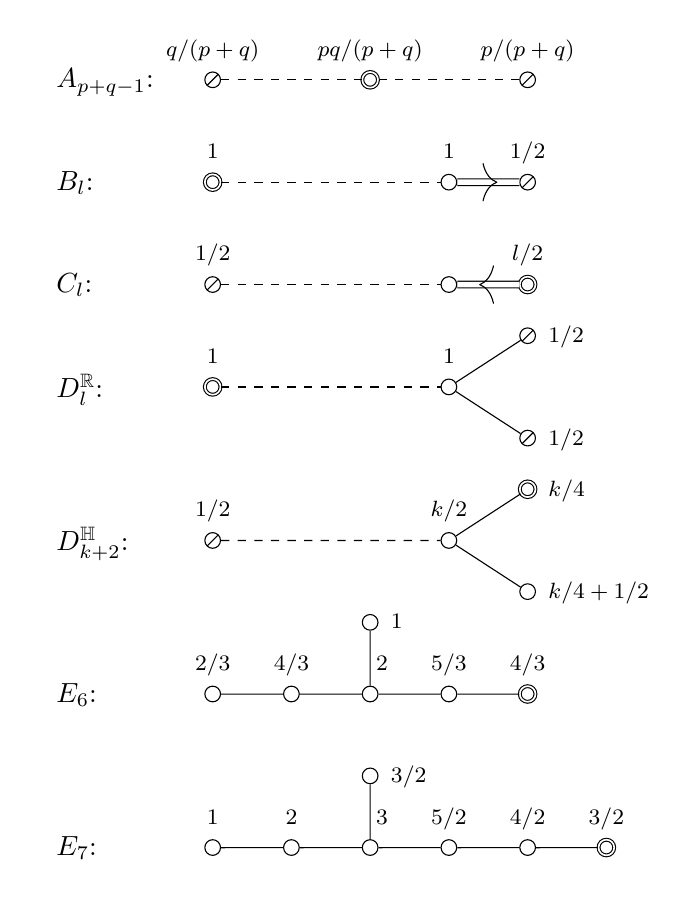
\begin{tikzpicture}[
  yscale=-1.3,
  every node/.style={draw,circle,inner sep=2pt},
  special/.style={double},
  symplectic/.style={forbidden sign},
  every label/.append style={rectangle,font=\footnotesize,
   inner sep=1ex,text depth=1pt},
  decoration={markings,mark=at position 0.7 with {\arrow{>}}},
  doubledynkin/.style={double distance=2pt,postaction=decorate}
  ]
  \node[draw=none] (Atext) [label=right:{\normalsize$A_{p+q-1}$:}] at (-1.25,0) {};
  \node[symplectic] (A1) [label={$q/(p+q)$}] at (1,0) {};
  \node[special] (Ap) [label={$pq/(p+q)$}] at (3,0) {};
  \node[symplectic] (Ak) [label={$p/(p+q)$}] at (5,0) {};
  \draw[dashed] (A1) -- (Ap);
  \draw[dashed] (Ap) -- (Ak);

  \node[draw=none] (Btext) [label=right:{\normalsize$B_{l}$:}] at (-1.25,1) {};
  \node[special] (B1) [label={$1$}] at (1,1) {};
  \node (Blm1) [label={$1$}] at (4,1) {};
  \node[symplectic] (Bl) [label={$1/2$}] at (5,1) {};
  \draw[dashed] (B1) -- (Blm1);
  \draw[doubledynkin] (Blm1) -- (Bl);

  \node[draw=none] (Ctext) [label=right:{\normalsize$C_{l}$:}] at (-1.25,2) {};
  \node[symplectic] (C1) [label={$1/2$}] at (1,2) {};
  \node (Clm1) at (4,2) {};
  \node[special] (Cl) [label={$l/2$}] at (5,2) {};
  \draw[dashed] (C1) -- (Clm1);
  \draw[doubledynkin] (Cl) -- (Clm1);

  \node[draw=none] (DRtext) [label=right:{\normalsize$D_{l}^{\RR}$:}] at (-1.25,3) {};
  \node[special] (DR1) [label={$1$}] at (1,3) {};
  \node (DRlm2) [label={$1$}] at (4,3) {};
  \node[symplectic] (DRlm1) [label=right:{$1/2$}] at (5,2.5) {};
  \node[symplectic] (DRl) [label=right:{$1/2$}] at (5,3.5) {};
  \draw[dashed] (DR1) -- (DRlm2);
  \draw (DRlm1) -- (DRlm2) -- (DRl);

  \begin{scope}[yshift=0.5cm]
   \node[draw=none] (DRtext) [label=right:{\normalsize$D_{k+2}^{\HQ}$:}] at (-1.25,4) {};
   \node[symplectic] (DR1) [label={$1/2$}] at (1,4) {};
   \node (DRlm2) [label={$k/2$}] at (4,4) {};
   \node[special] (DRlm1) [label=right:{$k/4$}] at (5,3.5) {};
   \node (DRl) [label=right:{$k/4+1/2$}] at (5,4.5) {};
   \draw[dashed] (DR1) -- (DRlm2);
   \draw (DRlm1) -- (DRlm2) -- (DRl);
  \end{scope}

  \node[draw=none] (DRtext) [label=right:{\normalsize$E_6$:}] at (-1.25,6) {};
  \node (E61) [label={$2/3$}] at (1,6) {};
  \node (E62) [label={$4/3$}] at (2,6) {};
  \node (E63) [label={\hbox{\hss\quad$2$}}] at (3,6) {};
  \node (E64) [label=right:{$1$}] at (3,5.3) {};
  \node (E65) [label={$5/3$}] at (4,6) {};
  \node[special] (E66) [label={$4/3$}] at (5,6) {};
  \draw (E61) -- (E62) -- (E63) -- (E64);
  \draw (E63) -- (E65) -- (E66);

  \begin{scope}[yshift=0.5cm]
   \node[draw=none] (DRtext) [label=right:{\normalsize$E_7$:}] at (-1.25,7) {};
   \node (E71) [label={$1$}] at (1,7) {};
   \node (E72) [label={$2$}] at (2,7) {};
   \node (E73) [label={\hbox{\hss\quad$3$}}] at (3,7) {};
   \node (E74) [label=right:{$3/2$}] at (3,6.3) {};
   \node (E75) [label={$5/2$}] at (4,7) {};
   \node (E76) [label={$4/2$}] at (5,7) {};
   \node[special] (E77) [label={$3/2$}] at (6,7) {};
   \draw (E71) -- (E72) -- (E73) -- (E74);
   \draw (E73) -- (E75) -- (E76) -- (E77);
  \end{scope}
 \end{tikzpicture}
\]
\end{minipage}\hfill% -}}}
\newdimen\curparindent
\curparindent=\parindent
\begin{minipage}{.41\textwidth} % {{{-3
 \parindent=\curparindent
 \divide\parindent by 3
 \multiply\parindent by 2
 \noindent
Legend (and comparison with \cite{Del_ShimVar}):
\begin{itemize}[leftmargin=\parindent]
 \item nodes are represented by circles~%
  \tikz \node[draw,circle,inner sep=2pt] {};
  (bars in \cite{Del_ShimVar});
 \item special nodes are represented by double circles~%
  \tikz \node[draw,circle,inner sep=2pt,double] {};
  (circled nodes in \cite{Del_ShimVar});
 \item symplectic nodes are represented by slashed circles~%
  \tikz \node[draw,circle,inner sep=2pt,forbidden sign] {};
  (underlined nodes in \cite{Del_ShimVar}).
\end{itemize}
(Symplectic nodes are defined below.)

The number next to a node $\omega$ is $\langle \mu,\omega \rangle$,
where $\mu$ is the cocharacter corresponding to the special node,
and $\omega$ is identified with the appropriate character.

In diagram~$A_{p+q-1}$ it is the $p$-th node that is special.
The diagram~$D_{k+2}^{\HQ}$ is required to satisfy $k + 2 \ge 5$.

The diagrams of type~$E_8$, $F_4$, and~$G_2$ do not occur:
they do not have special nodes.
The diagrams of type~$E_6$ and~$E_7$ do not have symplectic nodes.
\end{minipage} % -}}}

\begin{remark} % {{{-2
 There is a risk of confusing terminology:
 a \emph{connected component} of~$\Delta$ (or~$\Delta^\mu$)
 will always mean a connected component of the Dynkin diagram~$\Delta$
 (disregarding the $\Gal(\bar Q/Q)$-action);
 whereas an \emph{irreducible component} $\Delta_1^{\mu_1} \subset \Delta^\mu$
 is an irreducible $\Gal(\bar Q/Q)$-subset $\Delta_1$
 of connected components of~$\Delta$ and $\mu_1 = \Delta_1 \cap \mu$.
\end{remark}

\paragraph{} % {{{-2
\label{opposition-involution}
We recall the definition of the opposition involution on a Dynkin diagram.
Let $(R,\Phi)$ be an irreducible root system, and
let $\Delta \subset \Phi$ be a choice of positive simple roots.
Then $\Delta$ may be identified with
the vertices of the Dynkin diagram of~$(R,\Phi)$.
Let $W$ be the Weyl group of~$(R,\Phi)$, and
let $w_0$ be the longest element of the Weyl group (with respect to~$\Delta$).
Then $w_0(\Delta) = -\Delta$
and $-w_0$ defines an element~$\tau$ of $\Aut(\Delta) = \Out(G)$:
the \emph{opposition involution}.
This involution is non-trivial if and only if
$\Delta$ has type $A_k$ with $k \ne 1$, $D_k$ with $k$~odd, or $E_6$.

For Dynkin diagrams with multiple connected components
the opposition involution is defined as the disjoint union
of the componentwise opposition involutions.

\begin{definition} % {{{-2
 \label{symplectic-node}
	Retain the notation of the previous paragraph.
 Let $\mu \in \Delta$ be a special node.
 A node $\omega \in \Delta$ is called a \emph{symplectic} node
 (with respect to~$\mu$)
 if $\langle \mu, \omega + \tau(\omega) \rangle = 1$.
\end{definition}

\paragraph{} % {{{-2
The reasoning behind this terminology is best understood
in terms of Deligne's construction
(\cref{delignes-construction}, see also \S1.3 and~\S2.3 of~\cite{Del_ShimVar}):
the symplectic nodes correspond precisely to
the heighest weights of symplectic representations~$V$
such that $\mu$ defines a $\{-1,0,1\}$-grading on~$V$.

\begin{definition} % {{{-2
 \label{symplectic-nodes-deligne-dynkin-diagram}
 Let $\Delta^{\mu}$ be a Deligne--Dynkin diagram over a field~$Q$.
 The \emph{subset of symplectic nodes} attached to $\Delta^{\mu}$
 is the maximal subset $S \subset \Delta$ defined by the following conditions:
 \begin{enumerate}
  \item For every special node $\alpha \in \mu \subset \Delta$,
   let $\Delta_\alpha$ denote the connected component of~$\Delta$
   that contains~$\alpha$.
   Then $S \cap \Delta_\alpha$ consists only of
   symplectic nodes of~$\Delta_\alpha$ with respect to~$\alpha$.
   (See also \cref{table-deligne-dynkin-diagrams}.)
  \item The set $S$ is stable under the action of $\Gal(\bar Q/Q)$.
 \end{enumerate}
\end{definition}

\begin{definition} % {{{-2
 A Deligne--Dynkin diagram $\Delta^{\mu}$ over~$Q$ is \emph{symplectic}
 if for every irreducible component of $\Delta^{\mu}$
 its subset of symplectic nodes is non-empty.
\end{definition}

\paragraph{} % {{{-2
\label{abmotdeldyn}
The reason we study Deligne--Dynkin diagrams
is that we may naturally attach such a diagram to
any hyperadjoint abelian motive~$M$ over a field $K \subset \CC$.
Let $\Delta$ be the Dynkin diagram
of the adjoint linear algebraic group~$\GB(M)$ over~$\QQ$.
It naturally comes equipped with an action of $\Gal(\QQbar/\QQ)$.
Let $\mu \colon \Gm \to \GB(M)_\CC$ be the Hodge cocharacter.
By \S1.2.5 of~\cite{Del_ShimVar} this cocharacter may be identified
with a (non-empty) subset of special nodes $\mu \subset \Delta$.
In particular $\Delta^{\mu}$ is a populated Deligne--Dynkin diagram over~$\QQ$,
and we call it the \emph{Deligne--Dynkin diagram associated with $M$}.

\begin{theorem} % {{{-2
 If $M$ is a hyperadjoint abelian motive over a field $K \subset \CC$,
 then the Deligne--Dynkin diagram $\Delta^{\mu}$
 associated with~$M$ is symplectic.
 \begin{proof}
  Since $M$ is an abelian motive,
  there is an abelian variety $A/K$ such that $M \in \Tangen{\HH^1(A)}$.
  Therefore there is a quotient map $\GB(A) \onto \GB(M)$,
  and hence a map $\tilde\GG_{\mathrm{B}}(M) \to \GB(A)^{\der}$.
  The representation $\GB(A) \to \GL(\HB^1(A))$ is symplectic,
  and thus its restriction to $\tilde\GG_{\mathrm{B}}(M)$ is symplectic.
  In \S1.3 of~\cite{Del_ShimVar}, Deligne shows that this means
  that $\Delta^{\mu}$ is symplectic.
 \end{proof}
\end{theorem}

\paragraph{} % {{{-2
Let $M$ be a hyperadjoint abelian motive
over a finitely generated field $K \subset \CC$.
Let $\Delta^\mu$ be the Deligne--Dynkin diagram associated with~$M$.
Choose an embedding of $K$ into a $p$-adic field~$K_v$.
Let $C_v$ be the completion of an algebraic closure of~$K_v$.
By $p$-adic Hodge theory,
we know that there is a grading on $\Hp(M) \otimes_{\QQp} C_v$.
This determines a cocharacter~$\mu_{\HT}$ of
$\Gpc(M) \otimes_{\QQp} C_v \subset \GB(M) \otimes_\QQ C_v$,
the \emph{Hodge--Tate} cocharacter.

\begin{lemma} % {{{-2
 \label{hodge-tate-cochar-deldyn}
 Retain the notation of the previous paragraph.
 The conjugacy class of the cocharacter
 $\mu_{\HT} \colon \Gm[C_v] \to \GB(M) \otimes_\QQ C_v$
 is defined over~$\QQbar$ and coincides with the
 conjugacy class of the Hodge cocharacter
 $\mu \colon \Gm[\CC] \to \GB(M) \otimes_\QQ \CC$.
 In particular, $\mu_{\HT}$ determines the subset $\mu \subset \Delta$.
 \begin{proof}
  This follows from the comparison theorems
  between Betti cohomology, algebraic de~Rham cohomology,
  and $p$-adic \'etale cohomology.
 \end{proof}
\end{lemma}

\paragraph{The type of $\Delta^\mu$} % {{{-2
Let $\Delta^{\mu}$ be an irreducible populated Deligne--Dynkin diagram over~$Q$.
If $\Delta^{\mu}$ is symplectic,
the type of its connected components is classical:
$A_n$,~$B_n$, $C_n$, or~$D_n$.
Conversely, if the connected components of~$\Delta$
are of type $A_n$ (resp.~$B_n$, or~$C_n$),
then $\Delta^{\mu}$ is symplectic.
In this case we say that the \emph{type} of~$\Delta$
is $A_n$ (resp.~$B_n$ or~$C_n$).
The case where the connected components of~$\Delta$
are of type~$D_n$ requires more attention.

Assume that the connected components of~$\Delta$
are of type~$D_n$, with $n \ge 5$.
For every special node $\alpha \in \mu \subset \Delta$,
let $\Delta_\alpha$ be the connected component of~$\Delta$
that contains~$\alpha$.
The pair $(\Delta_\alpha, \alpha)$ is of type~$D_n^\RR$ or~$D_n^\HQ$
according to the diagrams listed in \cref{table-deligne-dynkin-diagrams}.
One readily verifies that $\Delta^{\mu}$ is symplectic if and only if
one of the following conditions holds:
\begin{itemize}
 \item for every special node~$\alpha$, the pair $(\Delta_\alpha, \alpha)$
  is of type $D_n^\RR$; or
 \item for every special node~$\alpha$, the pair $(\Delta_\alpha, \alpha)$
  is of type $D_n^\HQ$.
\end{itemize}
We say that $\Delta^\mu$ is of \emph{type}~$D_n^\RR$ (resp.~$D_n^\HQ$)
if the former (resp.~the latter) condition holds.

Now assume that the connected components of~$\Delta$ are of type~$D_4$.
Let $V$ be the subset of extremal nodes of~$\Delta$,
let $\bar\mu$ be the $\Gal(\bar Q/Q)$-closure of~$\mu$,
and let $S$ be the subset of symplectic nodes attached to $\Delta^{\mu}$.
Observe that $S \subset V$,
and $S$ meets every compontent of~$\Delta$ in $0$,~$1$, or~$2$ nodes.
(In other words, the degree of~$S$ over $\pi_0(\Delta)$ at most~$2$.)
In the former case, $S$ is empty, and $\Delta^{\mu}$ is not symplectic.
In the latter two cases $V = \bar\mu \sqcup S$, by the maximality of~$S$.
We say that $\Delta^{\mu}$ has \emph{type} $D_4^\RR$
if $\deg(\bar\mu) = 1$ and $\deg(S) = 2$,
while $\Delta^{\mu}$ has \emph{type} $D_4^\HQ$
if $\deg(\bar\mu) = 2$ and $\deg(S) = 1$.

\begin{remark} % {{{-2
 \label{type-remarks}
 Let $Q'/Q$ be a field extension,
 and let $\Delta^{\mu}$ be a Deligne--Dynkin diagram over~$Q$.
 By restricting the Galois action,
 one obtains a Deligne--Dynkin diagram $\Delta^{\mu}_{Q'}$ over~$Q'$.
 We make the following observations:
 \begin{enumerate}
  \item If $\Delta^{\mu}$ is irreducible or populated
   then this need not be true for $\Delta^{\mu}_{Q'}$.
   (Of course $\Delta^\mu_{Q'}$ will have
   irreducible components that are populated.)
  \item Related to the previous point:
   the subset of symplectic nodes attached to $\Delta^{\mu}_{Q'}$
   may be strictly larger then the subset of symplectic nodes of $\Delta^{\mu}$.
  \item If $\Delta^{\mu}$ is irreducible of type~$D_4^\HQ$
   then $\Delta^{\mu}_{Q'}$ may have irreducible components of type~$D_4^\RR$.
   On the other hand, if $\Delta^{\mu}$ is populated and symplectic,
   but not of type~$D_4^\HQ$,
   then every irreducible component of $\Delta^{\mu}_{Q'}$ that is populated
   must have the same type as $\Delta^{\mu}$.
 \end{enumerate}
\end{remark}

\begin{lemma} % {{{-2
 \label{locally-same-type}
 Let $\Delta^{\mu}$ be
 an irreducible symplectic populated Deligne--Dynkin diagram over~$\QQ$.
 Then there exists a prime number~$\ell$,
 and an irreducible component of $\Delta^{\mu}_{\QQl}$
 that has the same type as $\Delta^{\mu}$.
 \begin{proof}
  This is trivial, unless $\Delta^{\mu}$ has type~$D_4^\HQ$.
  In that case, let $\alpha \in \mu$ be a special node,
  and let $\Delta_\alpha$ be
  the connected component of~$\Delta$ that contains~$\alpha$.
  By assumption, the subset of symplectic nodes of $\Delta^{\mu}$
  meets $\Delta_\alpha$ in exactly one node~$s$.
  Label the remaining extremal node of~$\Delta_\alpha$ with $\beta$.
  By assumption we have $\bar\mu \cap \Delta_\alpha = \{\alpha,\beta\}$.
  By Chebotarev's density theorem
  there exists a prime number~$\ell$
  and an element $g \in \Gal(\QQlbar/\QQl)$ such that $g\alpha = \beta$.
  Let $\Delta'$ be the $\Gal(\QQlbar/\QQl)$-closure of $\Delta_\alpha$,
  and take $\mu' = \Delta' \cap \mu$.
  Then $(\Delta', \mu')$ has type~$D_4^\HQ$.
 \end{proof}
\end{lemma}

\paragraph{} % {{{-2
An \emph{isomorphism of Deligne--Dynkin diagrams}
$\phi \colon \Delta_1^{\mu_1} \to \Delta_2^{\mu_2}$ over a field~$Q$
is a $\Gal(\bar Q/Q)$-equivariant isomorphism
$\phi \colon \Delta_1 \to \Delta_2$ that maps $\mu_1$ onto~$\mu_2$.

Observe that there is a natural map
$\Isom(\Delta_1^{\mu_1},\Delta_2^{\mu_2})
\to \Isom(\pi_0(\Delta_1),\pi_0(\Delta_2))$,
and if $f \in \Isom(\pi_0(\Delta_1),\pi_0(\Delta_2))$,
then we write $\Isom_f(\Delta_1^{\mu_1},\Delta_2^{\mu_2})$
for the set of $\phi \in \Isom(\Delta_1^{\mu_1},\Delta_2^{\mu_2})$
such that $\pi_0(\phi) = f$.

\begin{lemma} % {{{-2
 Let $\Delta^{\mu}$ be
 an irreducible symplectic populated Deligne--Dynkin diagram over~$Q$.
 Let $\tau$ denote the opposition involution on~$\Delta$.
 Then
 \[
  \#\Aut_\id(\Delta^\mu) =
  \begin{cases}
   1 &\text{if $\Delta^\mu$ has type $A_1$,~$B_n$, $C_n$, $D_n^\HQ$,
   or $A_n$ and $\mu$ is not fixed by~$\tau$,}\\
   2 &\text{if $\Delta^\mu$ has type $D_n^\RR$, or $A_n$ ($n \ge 2$)
    and $\mu$ is fixed by~$\tau$.}
  \end{cases}
 \]
\end{lemma}

\begin{lemma} % {{{-2
 \label{locally-same-aut}
 Let $\Delta^{\mu}$ be
 an irreducible symplectic populated Deligne--Dynkin diagram over~$\QQ$.
 Then there exists
 an irreducible component $\Delta_\lambda^{\mu_\lambda}$ of $\Delta^{\mu}_{\QQl}$
 such that the natural map
 $\Aut_\id(\Delta^\mu) \to \Aut_\id(\Delta_\lambda^{\mu_\lambda})$
 is an isomorphism.
 \begin{proof}
  This follows immediately from \cref{locally-same-type}.
 \end{proof}
\end{lemma}

\paragraph{} % {{{-2
Let $\Delta^{\mu}$ be
an irreducible symplectic populated Deligne--Dynkin diagram over~$Q$.
The action of $\Gal(\bar Q/Q)$ on~$\Delta$
is determined by the action
a $\Gal(\bar Q/Q)$-closed subset $U(\Delta^\mu)$ of~$\Delta$.
Let $S$ be the subset of symplectic nodes of~$\Delta^{\mu}$.
\begin{itemize}
 \item If $(\Delta, \mu)$ is of type~$A_n$, we take~$U(\Delta^\mu) = S$.
 \item If $(\Delta, \mu)$ is of type~$B_n$, we take $U(\Delta^\mu) = S$.
 \item If $(\Delta, \mu)$ is of type~$C_n$, we take $U(\Delta^\mu) = \bar\mu$.
 \item If $(\Delta, \mu)$ is of type~$D_n^\RR$, we take $U(\Delta^\mu) = S$.
 \item If $(\Delta, \mu)$ is of type~$D_n^\HQ$,
  we take $U(\Delta^\mu) = \bar\mu$.
\end{itemize}
Note that the degree of $U(\Delta^\mu)$ over~$\pi_0(\Delta)$ is at most~$2$.

\paragraph{} % {{{-2
Let $\Delta_1^{\mu_1}$ and~$\Delta_2^{\mu_2}$ be two
irreducible symplectic populated Deligne--Dynkin diagrams over~$\QQ$.
Suppose there is a $\phi \in \Isom_f(\Delta_1^{\mu_1},\Delta_2^{\mu_2})$,
where $f$ is some $\Gal(\QQbar/\QQ)$-equivariant map
$\pi_0(\Delta_1) \to \pi_0(\Delta_2)$.
Let $\ell$ be a prime number.
Identify $\pi_0(\Delta_1)$ with $\Hom(E,\QQbar)$
for some number field~$E$.

We restrict the Galois action to $\Gal(\QQlbar/\QQl)$.
The irreducible components of~$(\Delta_1^{\mu_1})_{\QQl}$
are in a natural way indexed by the places~$\lambda$ of~$E$
that lie above~$\ell$.
In a similar manner, the maps~$f_\ell$ and~$\phi_\ell$
are the disjoint union of local components~$f_\lambda$ and~$\phi_\lambda$.
We will use this notation below.

\begin{proposition} % {{{-2
 \label{deldyn-local-global}
 Let $\Delta_1^{\mu_1}$ and~$\Delta_2^{\mu_2}$ be two
 irreducible symplectic populated Deligne--Dynkin diagrams over~$\QQ$.
 Suppose that there is an isomorphism
 $f \colon \pi_0(\Delta_1) \to \pi_0(\Delta_2)$
 and for each prime number~$\ell$ an element
 $\psi_\ell \in \Isom_f(\Delta_{1,\QQl}^{\mu_1},\Delta_{2,\QQl}^{\mu_2})$.
 Let $E$ be a number field such that $\Hom(E,\QQbar) = \pi_0(\Delta_1)$.

 Then there exists a $\phi \in \Isom_f(\Delta_1^{\mu_1},\Delta_2^{\mu_2})$
 and a finite place~$\lambda$ of~$E$
 such that $\phi_\lambda = \psi_\lambda$.
 \begin{proof}
  It suffices to prove the existence of~$\phi$;
  the second claim will follow automatically from \cref{locally-same-aut}.
  First of all, observe that $\Delta_1^{\mu_1}$ and~$\Delta_2^{\mu_2}$
  must have the same type, by \cref{type-remarks} and \cref{locally-same-type}.
  Next, we claim that there is an element in
  $\Isom_f(U(\Delta_1^{\mu_1}),U(\Delta_2^{\mu_2}))$.
  Indeed, since the degree of~$U(\Delta_i^{\mu_i})$ over~$\pi_0(\Delta_i)$
  is at most~$2$,
  it suffices (by Chebotarev's density theorem)
  to prove that these sets are locally isomorphic.
  If the type is not~$D_4^\HQ$,
  such local isomorphisms are provided
  by restricting the~$\psi_\ell$ to~$U(\Delta_1^{\mu_1})$.
  If the type is~$D_4^\HQ$,
  all $\psi_\ell$ will map $\mu_1$ to~$\mu_2$,
  but they need not all map $\Gal(\QQbar/\QQ)\cdot\mu_1$
  to~$\Gal(\QQbar/\QQ)\cdot\mu_2$.
  Suppose that $\psi_\lambda$ is a component of some~$\psi_\ell$
  for which $\psi_\lambda(\Gal(\QQbar/\QQ)\cdot\mu_1 \cap \Delta_{1,\lambda})$
  is not equal to $\Gal(\QQbar/\QQ)\cdot\mu_2 \cap \Delta_{2,\lambda}$.
  In that case the vertices of $\Delta_{i,\lambda}$
  form $4$~orbits under $\Gal(\QQlbar/\QQl)$
  and in particular there is an element in
  $\Isom_{f_\lambda}(U(\Delta_1^{\mu_1})_{\lambda},
  U(\Delta_2^{\mu_2})_{\lambda})$.
  As a consequence there is an element
  $\phi \in \Isom_f(\Delta_1, \Delta_2)$.
  It remains to prove that we can choose~$\phi$
  in such a way that it maps $\mu_1$ to~$\mu_2$.

  If $\Delta_1^{\mu_1}$ and $\Delta_2^{\mu_2}$
  are of type $A_1$,~$B_n$, $C_n$, or~$D_n^\RR$ then $\phi(\mu_1) = \mu_2$,
  hence there is nothing left to do.
  Now suppose that the type is $A_n$, with $n \ge 2$.
  If $\mu_1$ (and therefore $\mu_2$) is fixed
  under the opposition involution,
  then there is again nothing to do.

  Finally, suppose that the type is $D_n^\HQ$,
  or the type is $A_n$ and $\mu_i$ is not fixed by the opposition involution.
  Let $S_i$ be the subset of special nodes associated with~$\Delta_i^{\mu_i}$,
  and observe that $\phi(S_1) = S_2$.
  There is a unique non-trivial involution~$\tau_i \in \Aut_\id(\Delta_i)$
  such that $\tau_i(S_i) = S_i$.
  Now remark that $\phi \circ \tau_1 = \tau_2 \circ \phi$.
  Let $\alpha \in \mu_1$ be a special node that is not fixed under~$\tau_1$.
  We may assume that $\phi(\alpha) \in \mu_2$,
  by replacing $\phi$ with $\phi \circ \tau_1$ if necessary.
  
  We claim that $\phi(\mu_1) = \mu_2$.
  Indeed, suppose that $\alpha' \in \mu_1$ is a special node, and
  let $\Delta_{\alpha'}$ be the component of~$\Delta_1$ containing~$\alpha'$.
  There exists a $g \in \Gal(\QQbar/\QQ)$ such that
  \[
   \begin{cases}
    g\alpha = \alpha' &\text{if the type is~$D_4^\HQ$}\\
    g\alpha \in \Delta_{\alpha'} &\text{otherwise.}
   \end{cases}
  \]
  By Chebotarev's density theorem,
  we may assume that $g \in \Gal(\QQlbar/\QQl)$
  for some prime number~$\ell$.

  If the type is $D_4^\HQ$, then
  \[
   \phi(\alpha') = \phi(g\alpha) = g\phi(\alpha) = g\psi_\ell(\alpha)
   = \psi_\ell(g\alpha) = \psi_\ell(\alpha') \in \mu_2.
  \]
  Finally, if the type is not~$D_4^\HQ$, then we argue as follows:
  Let $\Delta_{1,\lambda}^{\mu_{1,\lambda}}$
  (resp.~$\Delta_{2,\lambda}^{\mu_{2,\lambda}}$)
  be the irreducible component of~$\Delta_{1,\QQl}^{\mu_1}$
  (resp.\ $\Delta_{2,\QQl}^{\mu_2}$)
  that contains~$\alpha$ (resp.~$\phi(\alpha)$).
  It is clear that $\phi_\lambda = \psi_\lambda$,
  and hence $\phi(\alpha') \in \mu_2$.
  This concludes the proof.
 \end{proof}
\end{proposition}

\section{Deligne's construction} % {{{-1
\label{delignes-construction}

\readme % {{{-2
Let $M$ be an irreducible hyperadjoint abelian motive over~$\CC$.
Proposition~2.3.10 of~\cite{Del_ShimVar} provides a recipe
to construct a complex abelian variety~$A$ (up to isogeny)
such that $M \cong \HH(A)^\ha$.
Deligne uses the language of Shimura data and Hodge theory.
We recall this construction,
using the terminology of abelian motives and Deligne--Dynkin diagrams.

\paragraph{Preparations} % {{{-2
Let $M$ be an irreducible hyperadjoint abelian motive over~$\CC$.
Write $G$ for the $\QQ$-simple adjoint group $\GB(M)$.
Let $E$ denote $\End(M)$,
and let $(\Delta,\mu)$ be the Deligne--Dynkin diagram associated with~$M$.
Recall that $E$ is a totally real field,
and that $\Hom(E,\QQbar) \cong \pi_0(\Delta)$.
Recall that $(\Delta,\mu)$ is symplectic,
and let $S$ be the subset of symplectic nodes associated with $(\Delta,\mu)$.

Let $\tilde G$ be the simply-connected cover of~$G$,
and for $s \in S$, let $V(s)$ be the representation of~$\tilde G_\CC$
whose heighest weight corresponds to~$s$.
The isomorphism class of $\bigoplus_{s \in S} V(s)$
is defined over~$\QQ$,
since $S$ is closed under the action of~$\Gal(\QQbar/\QQ)$.
Therefore, there exists a representation~$V$ of~$\tilde G$ over~$\QQ$
such that $V_\CC \cong \bigoplus_{s \in S} V(s)^{\oplus n}$
for suitable~$n$.

\paragraph{Choices} % {{{-2
\label{choices}
Now we fix three choices:
\begin{enumerate}
 \item Choose a totally imaginary quadratic extension $F/E$.
 \item Choose a partial CM~type~$\Phi$ for~$F$ relative to $(\Delta, \mu)$:
  a subset $\Phi \subset \Hom(F,\CC) = \Hom(F,\QQbar)$
  that maps 1-to-1 onto the complement of the image of~$\mu$
  in $\Hom(E,\QQbar) = \pi_0(\Delta)$.
 \item Choose a representation~$V$ of~$\tilde G$ as above.
\end{enumerate}

\paragraph{} % {{{-2
The Hodge cocharacter $h \colon \DelS \to G_\RR$ lifts to a map
$\tilde h \colon \tilde \DelS \to \tilde G_\RR$,
endowing~$V$ with a fractional Hodge structure.
The Hodge decomposition of~$V$ may be read of from
the diagrams in~\cref{table-deligne-dynkin-diagrams}.
If $s \in S$ lies in a component of~$\Delta$ that does not meet~$\mu$,
then the type of~$V(s)$ is $\{(0,0)\}$.
If $s$ lies in a component of~$\Delta$
that contains a special node $\alpha \in \mu$,
then the type of~$V(s)$ is $\{(r,-r), (r-1, 1-r)\}$
where $r = \langle s, \alpha \rangle$ is the rational number
that is written next the node~$s$
in the appropriate diagram in~\cref{table-deligne-dynkin-diagrams}.

\paragraph{} % {{{-2
Let $F_S$ denote the \'etale $E$-algebra
such that $\Hom(F_S, \QQbar) \cong S$ as $\Gal(\QQbar/\QQ)$-sets.
Observe that the fractional Hodge structure~$V$
is canonically an $F_S$-module:
the algebra~$F_S$ acts on~$V(s)$
via the embedding $F_S \into \QQbar \subset \CC$
that corresponds with $s \in S$.

We endow $F_S$ with a fractional pre-Hodge structure:
the component $\CC^{\{s\}}$ of $F_S \otimes_\QQ \CC \cong \CC^S$
is placed in bi-degree $(0,0)$
if $s$ lies in a component of~$\Delta$ that does not meet~$\mu$;
and $\CC^{\{s\}}$ is placed in bi-degree $(1-r,r)$
if $s$ lies in a component that does meet~$\mu$,
where $r$ is the rational number from the preceding paragraph.

\paragraph{} % {{{-2
In a similar fashion we endow the CM~field~$F$ with
a fractional pre-Hodge structure:
the component $\CC^\phi$ of $F \otimes \CC \cong \CC^{\Hom(F,\CC)}$
is placed in bi-degree
\[
 \begin{cases}
  (1,0) &\text{if $\phi \in \Phi$}\\ %TODO is this the right convention?
  (0,1) &\text{if $\bar\phi \in \Phi$}\\
  (0,0) &\text{otherwise.}
 \end{cases}
\]

\paragraph{} % {{{-2
\label{WF}
Write $W_F$ for $F \otimes_E F_S$, and
observe that $F \otimes_E F_S$ is a fractional Hodge structure of weight~$1$.
Note that $W_F$ is of CM~type,
since both~$F$ and $F_S$ are of CM~type.
Put $V' = W_F \otimes_{F_S} V$.
A computation shows that $V'$
is a Hodge structure of type $\{(1,0), (0,1)\}$.
It turns out that $V'$~is a polarisable Hodge structure
(see \cite{Del_ShimVar} for details).
Thus there is a complex abelian variety~$A$ (well-defined up to isogeny)
such that $\HB^1(A) \cong V'$.
Since $W_F$ is of CM~type,
we find that $\GB(V')^\ad = G$,
and therefore $\HH^1(A)^\ha = M$.

\paragraph{} % {{{-2
\label{tori-isog}
Write $T$ for the torus $\GB(A)^\ab = \GB(V')^\ab$.
Choose a faithful representation~$N$ of~$T$;
by the Tannakian formalism and \cref{hodge-is-motivated}
we may view~$N$ as an abelian CM~motive over~$\CC$.

Since $\GB(W_F)$ is a torus, and $\tilde G$ is almost simple,
the representation
\[
 \GB(W_F) \times \tilde G \to \Aut(V') = \Aut(W_F \otimes_{F_S} V)
\]
has a finite kernel.
In other words, the natural map
$\GB(W_F) \times \tilde G \to \GB(A)$ is an isogeny,
and so is the natural map $\GB(W_F) \to T$.

\paragraph{} % {{{-2
We end this section with a picture of the $\ell$-adic side of this story.
Let $K \subset \CC$ be a finitely generated field
such that the motive~$M$ and the abelian variety~$A$ are defined over~$K$.
We have the following diagram:
\[
 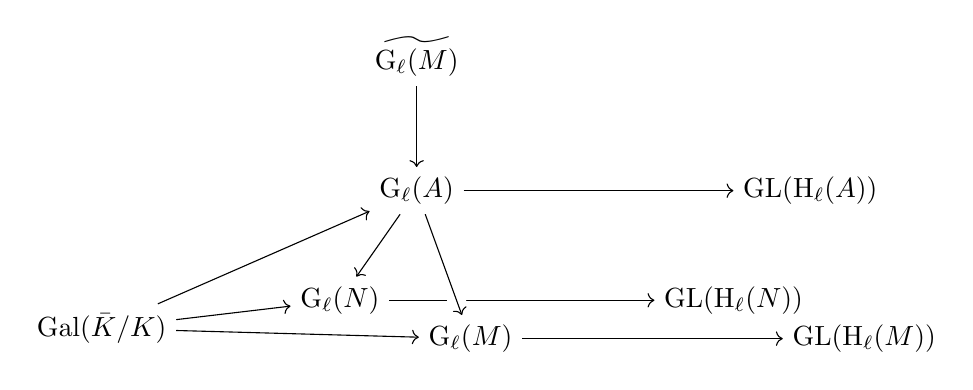
\begin{tikzpicture}[commutative diagrams/every diagram]
  \node (Gal) at (-4,-1.75) {$\Gal(\bar K/K)$};
  \node (GlA) at (0,0) {$\Gl(A)$};
  \node (GlMt) at (90:1.7) {$\widetilde{\Gl(M)}$};
  \node (GlN) at (55:-1.7) {$\Gl(N)$};
  \node (GlM) at (110:-2) {$\Gl(M)$};
  \node (HlA) at ($(0,0) +(5,0)$) {$\GL(\Hl(A))$};
  \node (HlN) at ($(55:-1.7) +(5,0)$) {\GL($\Hl(N))$};
  \node (HlM) at ($(110:-2) +(5,0)$) {$\GL(\Hl(M))$};
  \path[commutative diagrams/.cd, every arrow, every label]
  (GlM) edge (HlM)
  (GlN) edge (HlN)
  (GlA) edge (HlA)
  (GlMt) edge (GlA)
  (GlA) edge [commutative diagrams/crossing over] (GlM)
  (GlA) edge (GlN)
  (Gal) edge (GlA)
  (Gal) edge (GlN)
  (Gal) edge (GlM);
 \end{tikzpicture}
\]
Indeed, the map from $\Gal(\bar K/K)$ to $\Gl(A)$
exists by our assumption that $A$ is defined over~$K$.

\section{The main proposition} % {{{-1

\readme % {{{-2
In this section we prove the main technical result of this paper.
Its proof uses results of the previous three sections.

\begin{proposition} % {{{-2
 \label{mtc-product-abelian-motives}
 Let $M_1$ and~$M_2$ be two
 geometrically irreducible hyperadjoint abelian motives
 over a finitely generated field $K \subset \CC$.
 Assume that $\MTC(M_1)$ and $\MTC(M_2)$ are true, and
 assume that $\Gl(M_1 \oplus M_2)$ is connected for all prime numbers~$\ell$.
 If there exists a prime number~$\ell$
 such that $\Gl(M_1 \oplus M_2) \subsetneq \Gl(M_1) \times \Gl(M_2)$,
 then $\HB(M_1) \cong \HB(M_2)$ as Hodge structures.
\end{proposition}

\paragraph{} % {{{-2
\label{prp-strategy}
The proof of this \namecref{mtc-product-abelian-motives}
will take the rest of this section.
The strategy is as follows:
\begin{enumerate}
 \item First we prove that $\End(M_1) = \End(M_2)$.
 \item Next we show that $\Hl(M_1) \cong \Hl(M_2)$ for all primes~$\ell$.
 \item We use this (and \cref{deldyn-local-global})
  to show that $M_1$ and~$M_2$
  have isomorphic Deligne--Dynkin diagrams over~$\QQ$.
 \item After that we run Deligne's construction (\cref{delignes-construction})
  on the motives~$M_i$;
  this leaves us with two complex abelian varieties~$A_1$ and~$A_2$
  such that $M_{i,\CC} = \HH^1(A_i)^\ha$.
 \item We replace $K$ be a finitely generated extension,
  such that $A_1$ and~$A_2$ are defined over~$K$.
 \item By carefully tracing the $\ell$-adic counterpart of the construction
  we show that $A_1$ and~$A_2$ have isomorphic $\ell$-adic Tate modules.
 \item Finally, we apply Faltings's results to deduce that $A_1$ and~$A_2$
  are isogenous, which implies $\HB(M_1) \cong \HB(M_2)$.
\end{enumerate}
Sadly however, this strategy is slightly too optimistic.
It is not possible to work with the entire $\ell$-adic Galois representations,
and we will have to focus our attention on a suitable summand.
This makes the proof quite technical.

\paragraph{} % {{{-2
We first make some observations about~$M_1$ and~$M_2$.
For $i \in \{1,2\}$,
write $E_i$ for $\End(M_i)$, and
write $\Lambda_i$ for the set of finite places of~$E_i$.
For a prime number~$\ell$, let $\Lambda_{i,\ell}$
denote the set of places~$\lambda \in \Lambda_i$ that lie above~$\ell$.
Since $\MTC(M_i)$ holds, we know that
$\Glc(M_i) = \prod_{\lambda \in \Lambda_{i,\ell}}
\Res_{E_{i,\lambda}/\QQl} \Glambdac(M_i)$.
By assumption $\Gl(M_i) = \Glc(M_i)$,
and hence $\Glambda(M_i) = \Glambdac(M_i)$.
We also know that
$\Glambda(M_i)$ is a simple adjoint group over~$E_{i,\lambda}$,
once again, because $\MTC(M_i)$ holds.
Finally, remark that $\HH_{\Lambda_i}(M_i)$ is a
quasi-compactible system of representations,
by \cref{abelian-motive-quasi-compatible-realisations}.

Let $\ell$ be a prime number
such that $\Gl(M_1 \oplus M_2) \subsetneq \Gl(M_1) \times \Gl(M_2)$.
By Goursat's lemma this implies that there are
places $\lambda_1 \in \Lambda_{1,\ell}$
and $\lambda_2 \in \Lambda_{2,\ell}$
such that the projection of $\Gl(M_1 \oplus M_2)$ in
$\Res_{E_{1,\lambda_1}} \GG_{\lambda_1}(M_1) \times
\Res_{E_{2,\lambda_2}} \GG_{\lambda_2}(M_2)$
is the graph of an isomorphism of algebraic groups over~$\QQl$.
Hence there is a $\QQl$-linear isomorphism
$\psi \colon \HH_{\lambda_1}(M_1) \to \HH_{\lambda_2}(M_2)$
of Galois representations of~$K$.

Note that $\psi$ induces an isomorphism
$f \colon \End_{\Gal(\bar{K}/K)}(\HH_{\lambda_1}(M_1)) \to
\End_{\Gal(\bar{K}/K)}(\HH_{\lambda_2}(M_2))$,
and since these endomorphism algebras are commutative,
the isomorphism~$f$ does not depend on~$\psi$.
By \cref{recover-endomorphisms} we recover
$\lambda_i \colon E_i \into E_{i,\lambda_i} =
\End_{\Gal(\bar{K}/K)}(\HH_{\lambda_i}(M_i))$,
and therefore $\psi$ gives a canonical isomorphism
$f \colon E_1 \to E_2$ that identifies $\lambda_1$ with~$\lambda_2$.
Write $E$ for $E_1 = E_2$,
and write $\lambda$ for $\lambda_1 = \lambda_2$.
We conclude that $\Hlambda(M_1) \cong \Hlambda(M_2)$
as $\lambda$-adic Galois representations.

Write $\Lambda$ for the set of finite places of~$E$.
We assumed that $\Gl(M_{1} \oplus M_{2})$
is connected for all prime numbers~$\ell$.
Because $\Hlambda(M_1)$ and $\Hlambda(M_2)$
are semisimple and quasi-compatible,
\cref{quasi-compatible-semisimple-isomorphic}
shows that $\HLambda(M_1)$ and $\HLambda(M_2)$
are isomorphic quasi-compactible systems of representations.
We have now completed the first two steps of the strategy
outlined in \cref{prp-strategy}.

\paragraph{} % {{{-2
For $i = 1,2$, let $\Delta_i^{\mu_i}$
be the Deligne--Dynkin diagram associated with~$M_i$,
as in \cref{abmotdeldyn}.
Let $f \colon \pi_0(\Delta_1) \to \pi_0(\Delta_2)$,
that is defined by the canonical identifications
$\pi_0(\Delta_i) \cong \Hom(E,\QQbar)$.
Since $\HLambda(M_1)$ and $\HLambda(M_2)$ are isomorphic
as $E$-linear quasi-compactible systems of representations,
we get local isomorphisms
$\psi_\ell \in \Hom_f(\Delta_{1,\QQl},\Delta_{2,\QQl})$.
By \cref{hodge-tate-cochar-deldyn} we have
$\psi_\ell(\mu_1) = \mu_2$ for all~$\ell$.
Thus we may apply \cref{deldyn-local-global}
to obtain an isomorphism $\phi \in \Hom_f(\Delta_1^{\mu_1},\Delta_2^{\mu_2})$,
such that $\psi_\lambda = \phi_\lambda$ for some finite place~$\lambda$ of~$E$.

Let $S_i$ be the subset of symplectic nodes of~$\Delta_i^{\mu_i}$.
We will now apply Deligne's construction (see \cref{delignes-construction})
to the motives~$M_1$ and~$M_2$.
To do so, we have to make three choices, as in \cref{choices}:
\begin{enumerate*}[label=(\textit{\roman*})]
\item choose a totally imaginary quadratic extension $F/E$, and
\item endow it with a partial CM~type
 relative to $\Delta_1^{\mu_1} \stackrel{\phi}{=} \Delta_2^{\mu_2}$;
 finally,
\item choose the representations~$V_1$ and~$V_2$
 in such a way that they have the same dimension.
\end{enumerate*}
Let $F_{S_i}$ be an \'etale $E$-algebra such that
$\Hom(F_{S_i},\QQbar) \cong S_i$,
and write $W_{F,i}$ for $F \otimes_E F_{S_i}$.
Recall from \cref{WF} that $W_{F,i}$ caries a
fractional Hodge structure of weight~$1$ that is of CM~type.
The construction produces two complex abelian varieties~$A_1$ and~$A_2$,
such that $\HB(A_i) = W_{F,i} \otimes_{F_{S_i}} V_i$,
and $M_{i,\CC} = \HH^1(A_i)^\ha$.

\paragraph{} % {{{-2
As in \cref{tori-isog} let $T_i$ denote the torus $\GB(A_i)^\ab$.
Recall that the natural map $\GB(W_{F,i}) \to T_i$ is an isogeny.
The isomorphism~$\phi$ of Deligne--Dynkin diagrams
induces an isomorphism of fractional Hodge structure $W_{F,1} \cong W_{F,2}$.
Therefore there exists a torus~$T$,
together with isogenies $T_i \to T$.
Let $N$ be a faithful representation of~$T$.
By \cref{hodge-is-motivated} and the Tannakian formalism
we view $N$ as a complex motive.
Remark that $N$ is an abelian CM~motive.

Finally, we replace~$K$ with a finitely generated extension of~$K$
such that $A_1$,~$A_2$, $N$, and the maps $\GG(\HH^1(A_i)) \onto \GG(N)$
are defined over~$K$.
We are now ready for the two final steps in~\cref{prp-strategy}.

\paragraph{} % {{{-2
Let $\lambda$ be a finite place of~$E$ such that $\psi_\lambda = \phi_\lambda$,
and let $\ell$ be the residue characteristic of~$\lambda$.
Observe that $E$ acts on $M_i$,~$V_i$, $W_{F,i}$, and~$A_i$.
Let $\rho_i$ denote the Galois representation
$\Gal(\bar K/K) \to \Gl(A_i)(\QQl) \subset \GL(\Hl(A_i))(\QQl)$.
% We have the following diagram:
% \[
%  \begin{tikzpicture}[commutative diagrams/every diagram] % {{{-3
%   \def\cubel{.9}
%   % define a vanishing points
%   \coordinate (P1) at (-7,3.5);
%   \coordinate (P2) at (40,3.5);
%   % define a reference points
%   \coordinate (A1) at (0,1.5);
%   \coordinate (A2) at (0,-1.5);
%   \coordinate (A3) at ($(P1)!.7!(A2)$);
%   \coordinate (A4) at ($(P1)!.7!(A1)$);
%   \coordinate (Lc) at (barycentric cs:A1=1,A2=1,A3=1,A4=1);
%   \coordinate (Rc) at ($(P2)!\cubel!(Lc)$);

%   \node (Gal) at ($(Lc)!-1!(Rc)$) {$\Gal(\bar K/K)$};

%   \node (GlM1) at (A1) {$\Glambda(M_1)$};
%   \node (GlN1) at (A4) {$\Gl(N)$};
%   \node (GlA1) at (barycentric cs:Lc=-1.25,GlN1=1,GlM1=1) {$\Glambda(A_1)$};
%   \node (GlMt1) at ($(Lc)!1.5!(GlA1)$) {$\widetilde{\Glambda(M_1)}$};
%   \node (HlM1) at ($(P2)!\cubel!(GlM1)$) {$\GL(\Hlambda(M_1))$};
%   \node (HlN1) at ($(P2)!\cubel!(GlN1)$) {\GL($\Hl(N))$};
%   \node (HlA1) at ($(P2)!\cubel!(GlA1)$) {$\GL(\Hlambda(A_1))$};

%   \node (GlM2) at (A2) {$\Glambda(M_2)$};
%   \node (GlN2) at (A3) {$\Gl(N)$};
%   \node (GlA2) at (barycentric cs:Lc=-1.25,GlN2=1,GlM2=1) {$\Glambda(A_2)$};
%   \node (GlMt2) at ($(Lc)!1.5!(GlA2)$) {$\widetilde{\Glambda(M_2)}$};
%   \node (HlM2) at ($(P2)!\cubel!(GlM2)$) {$\GL(\Hlambda(M_2))$};
%   \node (HlN2) at ($(P2)!\cubel!(GlN2)$) {\GL($\Hl(N))$};
%   \node (HlA2) at ($(P2)!\cubel!(GlA2)$) {$\GL(\Hlambda(A_2))$};

%   \path[commutative diagrams/.cd, every arrow, every label]
%   (GlM1) edge (HlM1)
%   (GlN1) edge (HlN1)
%   (GlA1) edge (HlA1)
%   (GlM2) edge (HlM2)
%   (GlN2) edge (HlN2)
%   (GlA2) edge (HlA2)
%   (GlN1) edge [commutative diagrams/leftrightarrow] (GlN2)
%   (GlMt1) edge (GlA1)
%   (GlA1) edge [commutative diagrams/crossing over] (GlM1)
%   (GlA1) edge (GlN1)
%   (GlMt2) edge (GlA2)
%   (GlA2) edge (GlM2)
%   (GlA2) edge (GlN2)
%   (Gal) edge node {$\rho_1$} (GlA1)
%   (Gal) edge (GlN1)
%   (Gal) edge [commutative diagrams/crossing over] (GlM1)
%   (Gal) edge node[swap] {$\rho_2$} (GlA2)
%   (Gal) edge (GlN2)
%   (Gal) edge [commutative diagrams/crossing over] (GlM2)
%   (GlM1) edge [commutative diagrams/leftrightarrow,
%   commutative diagrams/crossing over] node[near end] {$\psi_\lambda$} (GlM2);
%  \end{tikzpicture} % -}}}
% \]
We make a table of all the data that is canonically identified
by $\phi_\lambda = \psi_\lambda$.
\begin{align*}
 \Glambda(M_1) &= \Glambda(M_2)
 &&\text{henceforth~$\Glambda$} \\
 \widetilde{\Glambda(M_1)} &= \widetilde{\Glambda(M_2)}
 &&\text{henceforth~$\widetilde{\Glambda}$} \\
 F_{S_1} \otimes_E E_\lambda &= F_{S_2} \otimes_E E_\lambda
 &&\text{as $E_\lambda$-algebras, henceforth~$F_{S,\lambda}$} \\
 W_{F,1} \otimes_E E_\lambda &= W_{F,2} \otimes_E E_\lambda
 &&\text{as $E_\lambda$-algebras, henceforth~$W_{F,\lambda}$} \\
 V_1 \otimes_E E_\lambda &= V_2 \otimes_E E_\lambda
 &&\text{as $\widetilde{\Glambda}$-representations
  with $F_{S,\lambda}$-action, henceforth~$V_\lambda$} \\
 \Hlambda(A_1) &= \Hlambda(A_2)
 &&\text{as $\widetilde{\Glambda}$-representations
  with $W_{F,\lambda}$-action, henceforth~$\Hlambda$} \\
\end{align*}
Let $G' \subset \GL(\Hlambda)$ be the subgroup
generated by the image of $\widetilde{\Glambda}$
and the image of $W_{F,\lambda}^\star$.
For $i = 1,2$, let $\rho_{i,\lambda}$ be
the $\lambda$-adic component of~$\rho_i$.
We may view $\rho_{i,\lambda}$ as a Galois representation on~$\Hlambda$,
and it takes values in~$G'$.
Observe that $\Glambda$ is the adjoint group of~$G'$,
and denote the projection with $\pi^\ad \colon G' \onto \Glambda$.
We note that $\pi^\ad \circ \rho_{i,\lambda}$ defines the Galois
representation on $\Hlambda(M_i)$,
and thus $\pi^\ad \circ \rho_{1,\lambda} = \pi^\ad \circ \rho_{2,\lambda}$.

\paragraph{} % {{{-2
Recall that we have an isogeny $p_i \colon \Gl(A_i)^\ab \to T_\ell = \Gl(N)$.
Denote the kernel of this isogeny with~$K_i$.
We also have a composition $\Gl(A_i) \onto \Glambda(A_i) \into G'$,
and therefore a map $\Gl(A_i)^\ab \to (G')^\ab$.
Let $K'_i$ be the image of~$K_i$ in~$(G')^\ab$ under this map,
and denote with $T'$ the quotient of $(G')^\ab$
by the finite group $K'_1 \cdot K'_2$.
Let $\pi^\ab \colon G' \onto T'$ be the natural projection map.
We claim that $\pi^\ab \circ \rho_{1,\lambda} = \pi^\ab \circ \rho_{2,\lambda}$.

Indeed, observe that $p_i \circ \rho_i$ defines
the Galois representation on~$\Hl(N)$,
which does not depend on~$i = 1,2$, since the motive~$N$ does not depend on~$i$.
If $q$ denotes the natural projection $T_\ell \onto T'$,
then $q \circ p_i \circ \rho_i = \pi^\ab \circ \rho_{i,\lambda}$.
This proves the claim that
$\pi^\ab \circ \rho_{1,\lambda} = \pi^\ab \circ \rho_{2,\lambda}$.

\paragraph{} % {{{-2
We are almost done!
Since $T'$ is a finite quotient of~$(G')^\ab$,
the group $\Gamma = \ker(\pi^\ad) \cap \ker(\pi^\ab)$ is a finite abelian group.
Define $\xi \colon \Gal(\bar \Gamma/\Gamma) \to G'(\QQl)$
via $\xi(g) = \rho_{1,\lambda}(g) \cdot \rho_{2,\lambda}(g)^{-1}$.
This map $\xi$ takes values in~$\Gamma$,
and is a homomorphism since $\Gamma$ is commutative.
We conclude that after replacing $K$ by a finite extension,
the Galois representations $\rho_1$ and~$\rho_2$ are the same.

This implies that $\Hlambda(A_1)$ and~$\Hlambda(A_2)$
are isomorphic as $\lambda$-adic Galois representations.
Another application of \cref{quasi-compatible-semisimple-isomorphic}
shows that $\HLambda(A_1)$ and~$\HLambda(A_2)$
are isomorphic $E$-rational quasi-compactible systems of representations.
Finally, Faltings's theorem
(Korollar~2 in~\S5 of~\cite{Fal83}, see also~\cite{Fal84})
implies that $A_1$ and~$A_2$ are isogenous.
Therefore $\HB(M_1) \cong \HB(M_2)$.
This concludes the proof of \cref{mtc-product-abelian-motives}.

\section{The main theorem} % {{{-1

\begin{lemma} % {{{-2
 \label{subgroup-surjective-projection-binary-products}
 Let $K$ be a field.
 For $i = 1, \dots, n$, let $G_i$ be a simple linear algebraic group over~$K$.
 Let $G$ be a subgroup of $G_1 \times \cdots \times G_n$,
 such that $G$ surjects onto $G_i$ for $1 \le i \le n$
 and $G$ surjects onto $G_i \times G_j$ for $1 \le i < j \le n$.
 Then $G = G_1 \times \cdots G_n$.
 \begin{proof}
  It suffices to prove the analogous statement for Lie algebras.
  This is precisely
  the lemma in step~3 on pages~790--791 of~\cite{Ribet}.
 \end{proof}
\end{lemma}

\begin{lemma} % {{{-2
	\label{mtc-finite-product-abelian-motives}
	Let $K \subset \CC$ be a finitely generated field.
	Let $M_{i}$, with $i \in I$, be a finite collection of
	irreducible hyperadjoint abelian motives over~$K$.
	Write $M = \bigoplus M_{i}$.
	If $\MTC(M_{i})$ is true for all $i \in I$,
	then $\MTC(M)$ is true.
	\begin{proof}
		By replacing $K$ with a finite extension,
		we may and do assume that $M_i$ is \emph{geometrically} irreducible
		for all $i \in I$.
		We also may and do assume that for $i,j \in I$
		we have $M_{i} \cong M_{j} \iff i = j$.
		Recall that there is a natural injection
		$\Gl(M) \into \prod_{i \in I} \Gl(M_{i})$
		and the image projects surjectively onto the factors $\Gl(M_{i})$.
		By \cref{mtc-product-abelian-motives},
		we know that if $i,j \in I$ are two different indices,
		then $\Gl(M_{i} \oplus M_{j}) \cong \Gl(M_{i}) \times \Gl(M_{j})$;
		in other words,
		$\Gl(M)$ surjects onto $\Gl(M_{i}) \times \Gl(M_{j})$.
		By \cref{subgroup-surjective-projection-binary-products}
		we conclude that $\Gl(M) \cong \prod_{i \in I} \Gl(M_{i})$.
	\end{proof}
\end{lemma}

\begin{theorem} % {{{-2
	\label{mtc-abelian-motives-tannakian-subcategory}
	Fix a finitely generated field $K \subset \CC$.
	Let $\mathcal{M}_{K} \subset \Mot_{K}$ be the full subcategory
	of \emph{abelian} motives for which the Mumford--Tate conjecture is true.
	Then the category~$M_{K}$ is a Tannakian subcategory of $\Mot_{K}$.
	\begin{proof}
		The category~$\Mot_{K}$ is semisimple,
		so subquotients are direct summands.
		It is clear that the subcategory~$\mathcal{M}_{K}$
		is closed under duals, tensor powers, and direct summands.
		Let $M_{1}$ and~$M_{2}$ be two objects in~$\mathcal{M}_{K}$.
		We need to show that $M_{1} \oplus M_{2}$
		and $M_{1} \otimes M_{2}$ are objects in $\mathcal{M}_{K}$.
		Observe that $M_{1} \otimes M_{2}$ is a direct summand of
		$(M_{1} \oplus M_{2})^{\otimes 2}$.
		Thus we are done if we show that the Mumford--Tate conjecture is true for
		$M = M_{1} \oplus M_{2}$.
		By \cref{mtc-adjoint-motive} we may assume that $M$ is hyperadjoint.
		Write $M = \bigoplus_{i \in I} M'_{i}$,
		with the $M'_{i}$ hyperadjoint.
		Now the result follows from \cref{mtc-finite-product-abelian-motives}.
	\end{proof}
\end{theorem}

\begin{theorem} % {{{-2
 \label{mtcaxa}
 Let $K$ be a subfield of~$\CC$.
 Let $A_i$, $i \in I$, be a finite collection of abelian varieries over~$K$,
	and write $A = \prod_{i \in I} A_i$.
 Assume that $\MTC(A_i)$ is true for all $i \in I$.
 Then $\MTC(A)$ is also true.
 \begin{proof}
  This is an immediate consequence of
  \cref{mtc-abelian-motives-tannakian-subcategory}.
 \end{proof}
\end{theorem}


% {{{-1 Footer
\printbibliography

\end{document}
